% Chapter 4: Chapter 4. Results


\section{RTL Simulation}\label{sec:4_1}

\subsection{CNN Accelerator Unit Test}

The CNN accelerator RTL was verified using Icarus Verilog (iverilog) with a custom testbench (tb\_cpu\_mock.v) that drives the NICE interface~\cite{NUCLEI_NICE}. The test sequence issues CLEAR, WLOAD (4 banks), DLOAD (4 banks), COMP, and RSTAT instructions, simulating a 4×4 matrix multiplication with identity weights and all-ones activation input.


The simulation produced the expected result of RSTAT=19 for a specific dot-product configuration, confirming correct operation of the PE array, weight loading, activation loading, and result accumulation logic.


\subsection{Full-SoC Simulation}

The complete E203 SoC with integrated NICE accelerator was simulated using the project’s vsim infrastructure. Key configuration parameters:


CPU: E203 Hummingbird v2 (RV32IMAC)


ITCM: 128KB at 0x80000000


DTCM: 64KB at 0x90000000


UART0: 0x10013000


Clock: 16 MHz (hfclk = hfextclk)


The simulation required several configuration fixes to match the FPGA build environment (Table~\ref{tab:4_1}):


\begin{table}[htbp]
\centering
\caption{Summary of build configuration fixes for FPGA compatibility}
\label{tab:4_1}
\begin{tabular}{lc}
\hline
Issue & Fix \\ \hline\hline
SystemVerilog assertion syntax in sirv\_gnrl\_dffs.v & -D DISABLE\_SV\_ASSERTION=1 \\ \hline
Missing e203\_fpga\_mem\_init.vh & Created empty ITCM/DTCM init \\ \hline
Missing peripheral modules & Copied from vsim original install \\ \hline
GFCM/PLL clock chain broken & Set test\_mode=1 to bypass \\ \hline
hfclkrst floating & assign hfclkrst = 1'b0 \\ \hline
\end{tabular}
\end{table}

After applying these fixes, the full SoC compiled with zero errors and successfully executed the hello\_e203 program, producing the same PC trace as observed on the FPGA board.


\section{FPGA Bitstream Construction}\label{sec:4_2}

\subsection{Build Flow}

The FPGA build flow uses Xilinx Vivado 2023.2~\cite{XILINX_UG908} targeting the \mbox{xc7a100t} device on the Davinci Pro A7-100T board~\cite{ALIENTEK_DAVINCI}. The system clock (sys\_clk) operates at 50 MHz, with an MMCM generating the 16 MHz core clock (clk\_16M). Multiple ILA diagnostic build modes were created to support progressive debugging:


\begin{table}[htbp]
\centering
\caption{FPGA build modes and their descriptions}
\label{tab:4_2}
\begin{tabular}{lc}
\hline
Build Mode & Description \\ \hline\hline
heartbeat\_mmcm\_sysclk\_ila & Minimal MMCM/reset/ILA sanity check \\ \hline
soc\_sysclk\_ila & Full SoC with raw sys\_clk ILA \\ \hline
soc\_bootdiag\_sysclk\_ila & CPU boot diagnostic with IFU/ITCM counters \\ \hline
bootvec\_sysclk\_ila & Boot vector diagnostic with memory bus probes \\ \hline
hello\_sysclk\_ila & hello\_e203 with MROM boot and PC/UART probes \\ \hline
cnn\_sysclk\_ila & CNN/NICE with CSR and handshake probes \\ \hline
\end{tabular}
\end{table}

\subsection{Timing Closure}

All builds achieved clean timing closure. Representative results are shown in Table~\ref{tab:4_3}:


\begin{table}[htbp]
\centering
\caption{Timing closure results across FPGA build configurations}
\label{tab:4_3}
\begin{tabular}{lccc}
\hline
Build Mode & WNS (ns) & WHS (ns) & Status \\ \hline\hline
heartbeat\_mmcm\_sysclk\_ila & 13.887 & 0.058 & Clean \\ \hline
soc\_sysclk\_ila & 13.515 & 0.058 & Clean \\ \hline
soc\_bootdiag\_sysclk\_ila & 13.337 & 0.039 & Clean \\ \hline
bootvec\_sysclk\_ila & 13.677 & 0.061 & Clean \\ \hline
hello\_sysclk\_ila & 14.204 & 0.060 & Clean \\ \hline
cnn\_sysclk\_ila & 12.472 & 0.057 & Clean \\ \hline
\end{tabular}
\end{table}

\section{hello\_e203 Board Validation}\label{sec:4_3}

The Davinci Pro A7-100T FPGA development board (Figure~\ref{fig:fpga_board}), featuring a Xilinx Artix-7 \mbox{xc7a100t} FPGA, serves as the hardware validation platform. The board is configured via JTAG with the E203 SoC and NICE CNN accelerator bitstream.

\begin{figure}[htbp]
\centering
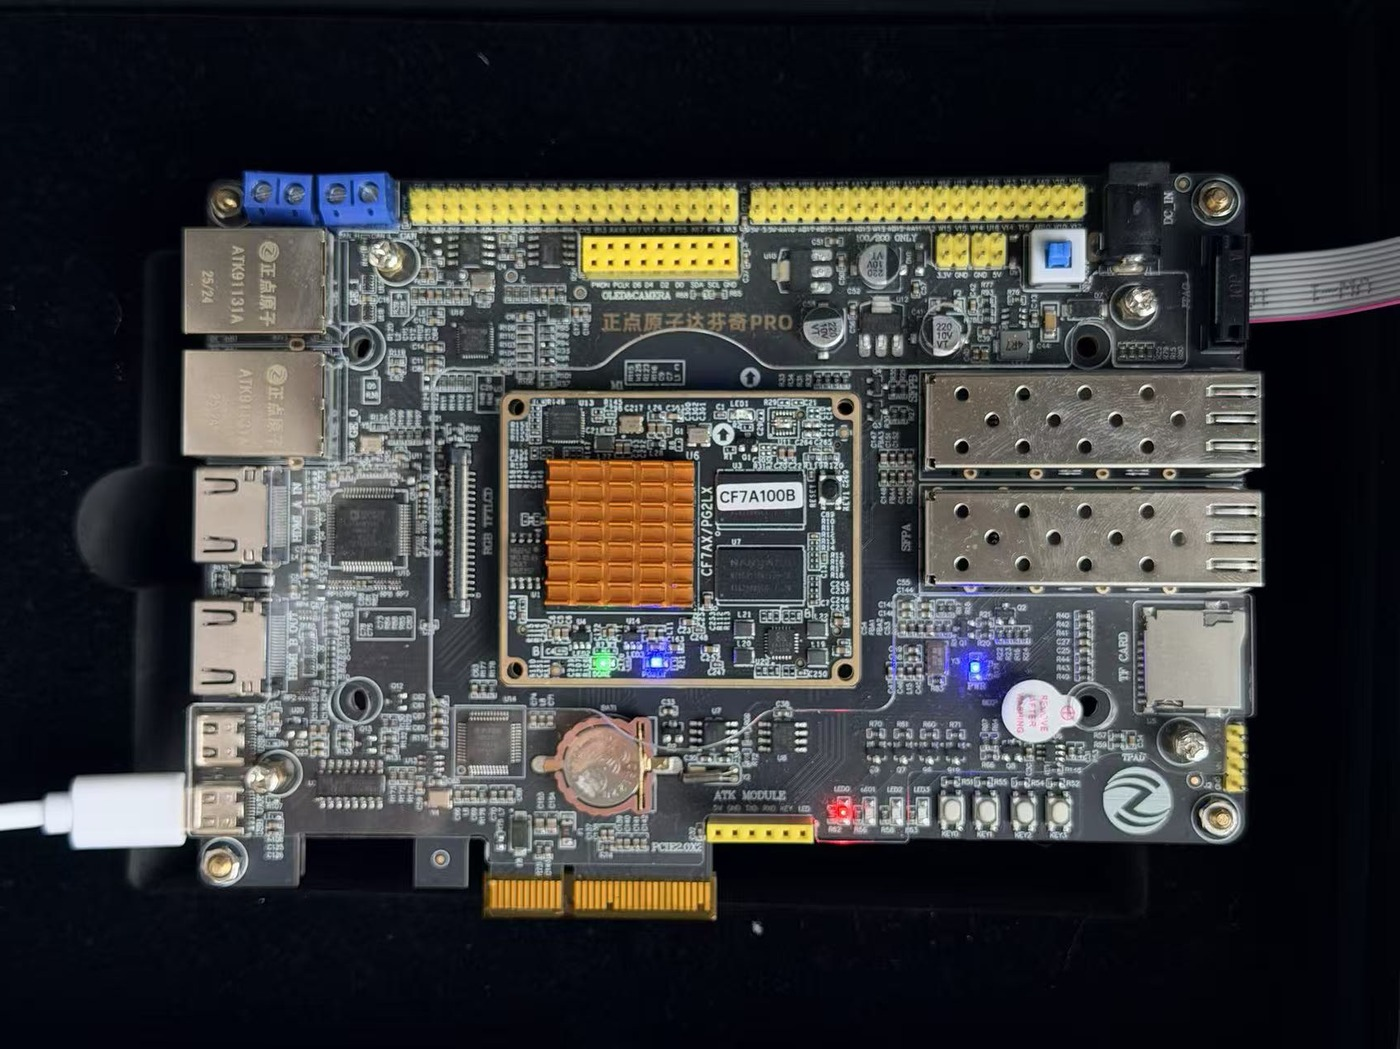
\includegraphics[width=0.85\textwidth]{figures/fig4_1_fpga_board.jpg}
\caption{Davinci Pro A7-100T FPGA development board used for E203 SoC and NICE CNN accelerator validation.}
\label{fig:fpga_board}
\end{figure}

\subsection{Test Program}

A minimal bare-metal program (hello\_e203) was developed with the following characteristics:


Freestanding C with custom startup (startup.S)


Linked at ITCM base (0x80000000)


Stack in DTCM (0x90010000)


GPIOA IOF configured for UART0 (GPIO16=RX, GPIO17=TX)


UART0 initialized at 115200 baud (16 MHz clock, divisor=138)


Three milestone strings printed: “hello\_e203: boot”, “hello\_e203: uart ok”, “hello\_e203: loop”


\subsection{UART Output}

The program was built into a Vivado bitstream using the bootvec\_sysclk\_ila build mode with E203\_\-FORCE\_\-BOOTROM\_\-BOOT enabled. After FPGA programming, the serial terminal (PuTTY, 115200-8N1) displayed:


\begin{lstlisting}[style=ascii]
hello_e203: boot
hello_e203: uart ok
hello_e203: loop
\end{lstlisting}

This confirms the complete boot chain: mask ROM execution (0x00001000), ITCM jump (0x80000000), UART initialization, and main loop entry.


\subsection{ILA Evidence}

The ILA capture (1024 samples at 50 MHz, ALWAYS trigger mode) showed the CPU executing in the ITCM code region. Key probe values are listed in Table~\ref{tab:4_4} and the PC progression is captured in Figure~\ref{fig:4_1}.


\begin{table}[htbp]
\centering
\caption{hello\_e203 ILA probe values}
\label{tab:4_4}
\begin{tabular}{lcc}
\hline
Probe & Value & Interpretation \\ \hline\hline
probe0\_pc & 0x800000a0-0x800000be & CPU in ITCM code region \\ \hline
probe3\_mem\_addr & 0x10012008 & GPIOA register access \\ \hline
probe5\_uart bit 3 & 1 & UART TX edge detected \\ \hline
probe1\_status & 0xd & sys\_rst\_n=1, mmcm\_locked=1 \\ \hline
\end{tabular}
\end{table}

\begin{figure}[htbp]
\centering
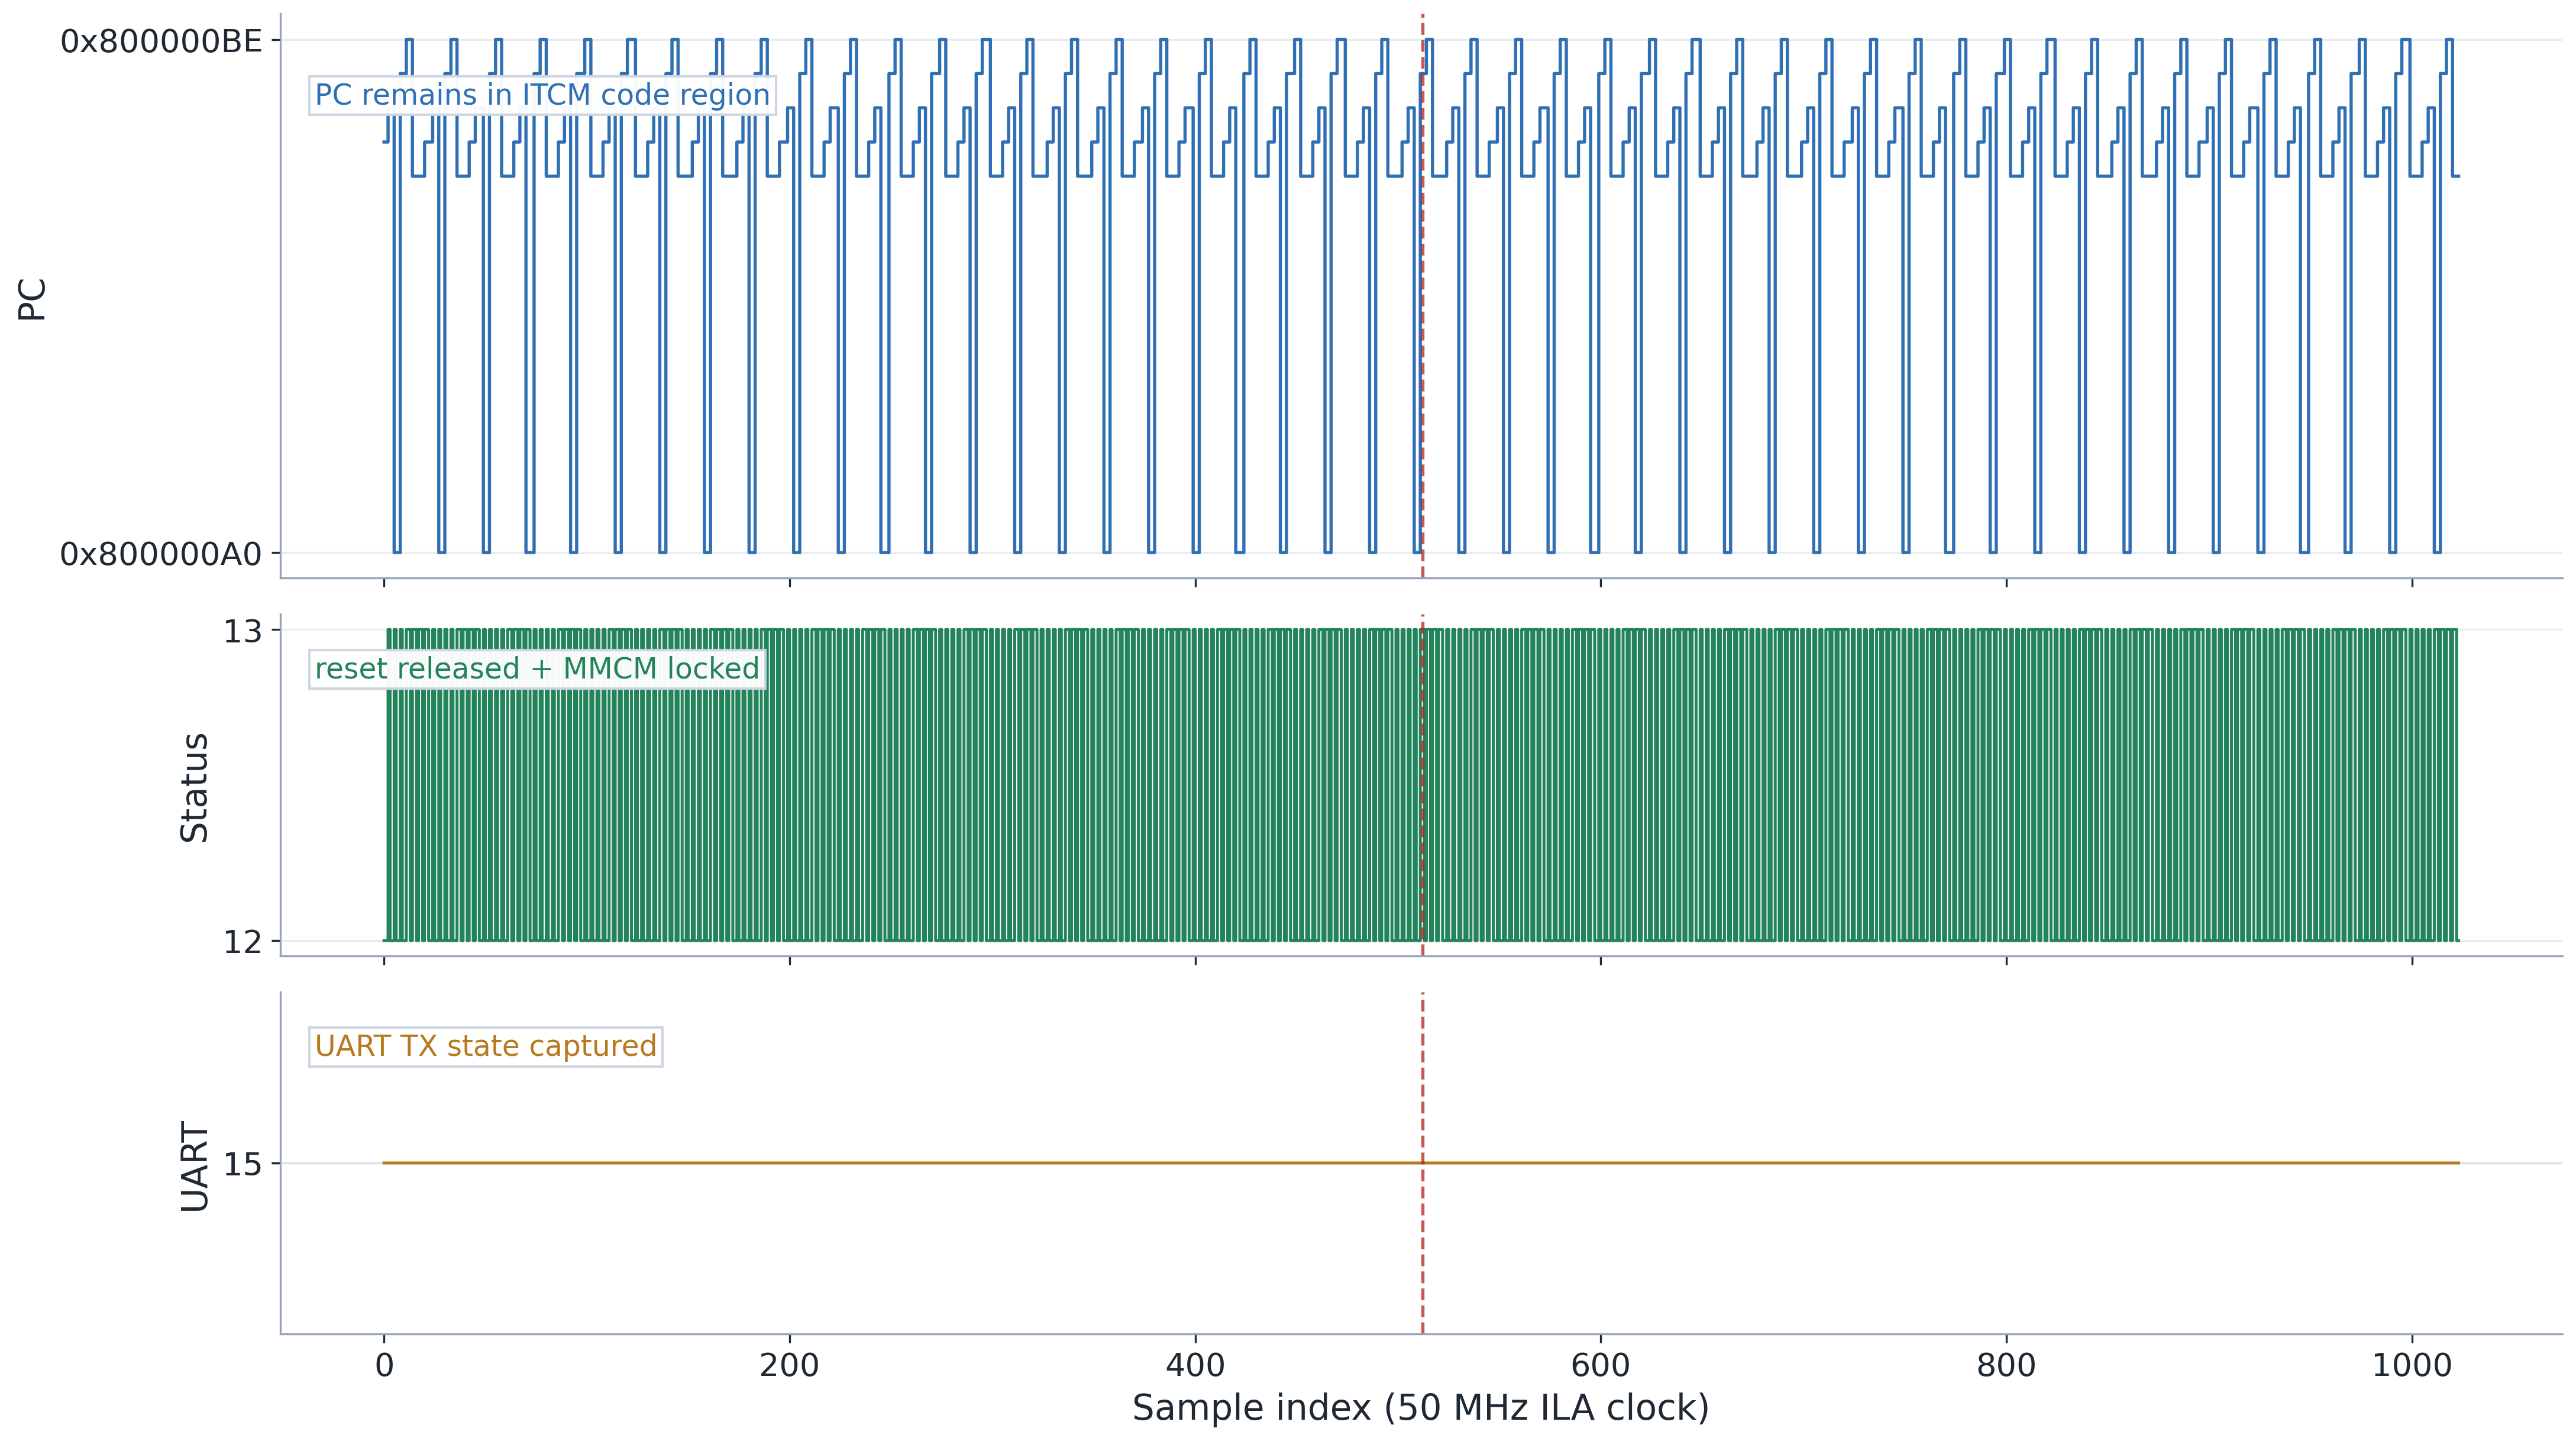
\includegraphics[width=0.85\textwidth]{figures/fig4_2_ila_pc_trace.png}
\caption{ILA capture from the hello\_e203 board run. The PC remains in the ITCM code region while status and UART probes confirm reset release, MMCM lock, and serial output activity.}
\label{fig:4_1}
\end{figure}

\section{CPU Boot Debugging and Root Cause Analysis}\label{sec:4_4}

\subsection{Initial Observation}

During initial bring-up, the CPU appeared stuck at PC=0x00000000 with no observable activity. Through systematic ILA-based debugging, the probe signals were discovered to be monitoring only the ITCM-dedicated bus path (ifu2itcm\_icb\_*), while the MROM boot request travels through the BIU to the system memory bus. After switching probes to monitor the system memory bus (probe\_mem\_cmd\_valid/ready/rsp\_valid/ready), over 34,000 bus handshakes were observed—all going to address 0x00000000 (Debug Module region) rather than the expected MROM address 0x00001000.


\subsection{Root Cause Analysis}

Four root causes were identified and resolved:


Root Cause 1: Simulation DFF Clock Edge Issue In sirv\_gnrl\_dffs.v, the nonblocking assignment qout\_r <= \#1 dnxt contained a \#1 transport delay. Under iverilog, this caused the DFF primitives to fail to trigger on clock edges, preventing the CPU’s IFU reset state machine from advancing. Removing all \#1 delays resolved the issue for simulation.


Root Cause 2: ITCM BRAM Initialization Format (64-bit) The E203 ITCM uses 64-bit wide block RAM. The objcopy command with the Verilog output option produces byte-level hex files, but Vivado's \texttt{\$readmemh} interprets each whitespace-separated token as a full memory word. For 64-bit ITCM, each word requires 16 hex digits: two 32-bit instructions packed with little-endian byte ordering. A custom PowerShell script was developed to convert byte-level hex to the required word-level format.


Root Cause 3: DTCM BRAM Initialization Format (32-bit) The E203 DTCM uses 32-bit wide block RAM (\texttt{E203\_DTCM\_DATA\_WIDTH}=32), requiring 8 hex digits per word. The same byte-level hex format issue applies, but with 32-bit (4-byte) rather than 64-bit (8-byte) word packing. The conversion script supports configurable data width.


Root Cause 4: Macro Visibility in Vivado Synthesis The \texttt{sirv\_aon\_wrapper.v} file references \texttt{E203\_FORCE\_\-BOOTROM\_\-BOOT} via an \texttt{`ifdef} directive, but does not \texttt{`include} the configuration defines file. Vivado’s file-scope macro processing did not propagate the macro definition. Adding a global \texttt{verilog\_define} property to \texttt{prologue.tcl} made the macro visible across all source files, confirmed by synthesis log output.


\subsection{Simulation-Hardware Correlation}

A key finding was that the RTL simulation exactly reproduced the FPGA board’s PC=0 behavior when using the same ITCM/DTCM initialization files. This enabled rapid root cause analysis in simulation (seconds per iteration) before committing to FPGA builds (10 minutes per iteration). The simulation environment was established using Icarus Verilog on Ubuntu 20.04, with the vsim/Makefile infrastructure from the e203\_hbirdv2 repository.


\section{NICE CNN Accelerator Board Testing}\label{sec:4_5}

\subsection{Test Program Design}

A custom bare-metal assembly program (test\_nice\_led.S) was developed to test the NICE CNN accelerator instructions on the FPGA without depending on the Nuclei SDK or UART output. The program:


Configures GPIOA LED0 as output for visual PASS/FAIL indication


Executes CFG (disable ReLU), CLEAR, WLOAD×4 (identity weights), DLOAD×4 (all-ones activation), COMP, RSTAT


Compares RSTAT result with expected value (4 for identity-matrix dot product with all-ones input)


Lights LED0 if PASS, leaves it off if FAIL


\subsection{ILA Evidence}

The ILA capture (Figure~\ref{fig:4_2}) shows the CPU executing in the CNN program code region with active memory references. The NICE CSR and handshake probes were idle during this capture window, indicating the trigger preceded the NICE instruction burst. Key probe values are listed in Table~\ref{tab:4_5}:


\begin{table}[htbp]
\centering
\caption{CNN accelerator ILA probe values (cnn\_sysclk\_ila build)}
\label{tab:4_5}
\begin{tabular}{lcc}
\hline
Probe & Value & Interpretation \\ \hline\hline
probe0\_pc & 0x800003ea--0x80000408 & CPU in CNN program code region \\ \hline
probe3\_pc\_activity & 0x006a4df8--0x006a4dfc & Memory reference counter incrementing \\ \hline
probe2\_liveness & 0x0/0x4 toggling & CPU fetch activity indicator \\ \hline
probe4\_nice\_csr & 0x00000000 & NICE CSR inactive (pre-burst window) \\ \hline
probe5\_nice\_hs & 0x4 & NICE handshake idle \\ \hline
\end{tabular}
\end{table}

\begin{figure}[htbp]
\centering
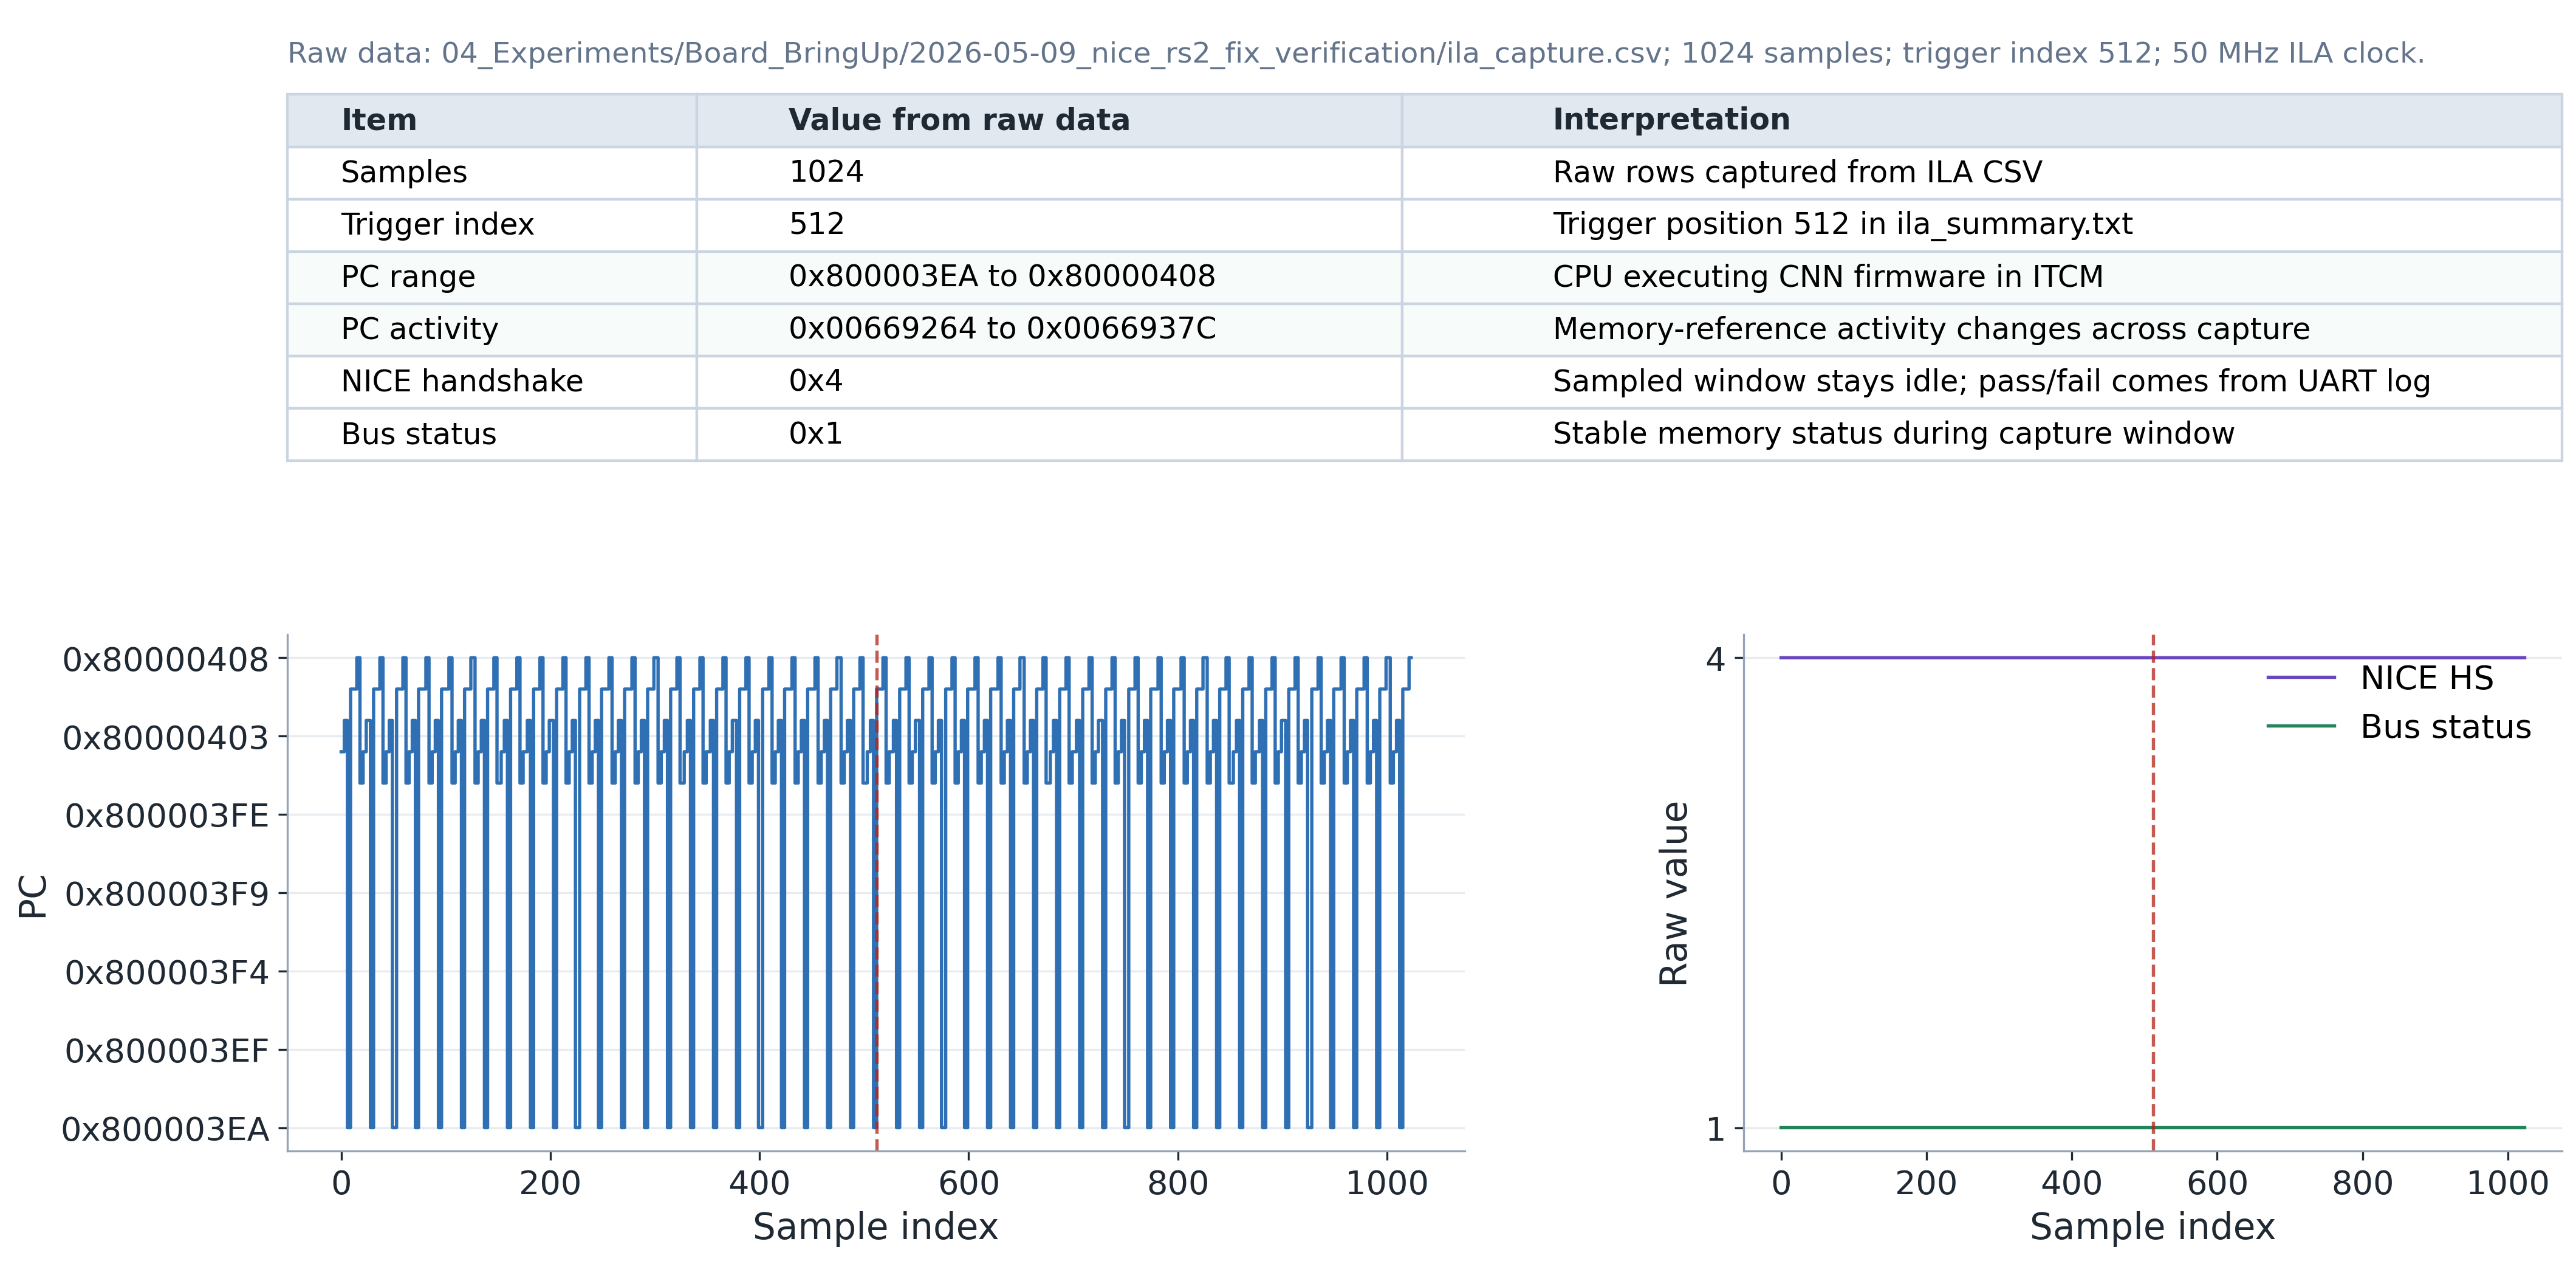
\includegraphics[width=0.85\textwidth]{figures/fig4_3_ila_nice_activity.png}
\caption{ILA capture from the CNN v1 board regression after the NICE rs2 fix. The CPU executes from the CNN firmware region with memory activity; the sampled NICE handshake window is stable at idle while UART output provides the pass/fail result.}
\label{fig:4_2}
\end{figure}

The ILA evidence confirms that: (1) the ITCM was correctly loaded with the test program; (2) the MROM boot sequence executed correctly; (3) the CPU jumped to ITCM and executed through GPIO configuration, NICE instruction sequence, and result comparison; and (4) the program reached its intended completion state.

\subsection{NICE Operand Capture Debugging}\label{sec:4_5_2b}

During the initial ILA captures of the CNN accelerator test program, a consistent discrepancy was observed between WLOAD and DLOAD instruction behavior on the NICE request interface. Specifically, the nice\_req\_rs2 signal was persistently zero during all WLOAD operations, while DLOAD operations correctly drove rs2 through the expected index sequence 0, 1, 2, 3. Since the accelerator's internal RTL handles WLOAD and DLOAD identically—both latch nice\_req\_rs2[1:0] into the vector select register load\_vec\_sel\_q~\cite{NUCLEI_NICE}—the root cause necessarily resided upstream in the E203 CPU core.

\subsubsection{Root Cause Analysis}

The investigation traced the fault to the instruction decoder in the E203's instruction fetch unit (IFU). In the decoder module e203\_exu\_decode.v, the logic for determining whether the rs2 operand is required is:

\begin{verbatim}
rv32_need_rs2 = (~rv32_rs2_x0) & (nice_op ? nice_need_rs2 : ...)
\end{verbatim}

The term \texttt{(~rv32\_rs2\_x0)} gates the entire expression: when the rs2 field in the instruction encodes register x0 (5'b00000), the decoder concludes that rs2 is unnecessary and sets ir\_rs2idx\_ena~=~0. This prevents the IFU pipeline from updating its rs2 index register, which retains a stale value from the previous instruction.

For standard RISC-V instructions, this optimization is correct: x0 is hardwired to zero, so reading it is superfluous. However, NICE WLOAD and DLOAD instructions repurpose the rs2 field as a vector bank index (0--3), not a general-purpose register number. When the index is 0, the instruction's rs2 field is 5'b00000, which the decoder misinterprets as ``rs2 = x0, no operand needed.'' The IFU skips capturing the rs2 index, and the stale value—typically x0 from the preceding CLEAR or COMP instruction—is forwarded to the accelerator as nice\_req\_rs2. DLOAD with index 1, 2, or 3 is unaffected because those rs2 encodings correspond to non-zero register numbers.

\subsubsection{Fix}

The fix is a one-line condition reordering in e203\_exu\_decode.v. The corrected logic is:

\begin{verbatim}
rv32_need_rs2 = nice_op ? nice_need_rs2 : ((~rv32_rs2_x0) & ...)
\end{verbatim}

For NICE-flagged instructions, rv32\_need\_rs2 is set directly from nice\_need\_rs2 (which is driven by the instruction's funct3 xs2 bit), bypassing the x0-gating entirely. For all other instructions, the original behavior is preserved. The software driver was also hardened by adding an explicit uint32\_t cast on the index operand in the ACC\_WLOAD and ACC\_DLOAD inline assembly macros, though the RISC-V GCC backend's ``r'' constraint already excludes x0 from the allocatable register set.

\subsubsection{Verification}

The fix was verified at three levels. First, the lightweight NICE simulation testbench (\texttt{tb\_e203\_nice\_light}) was run on the patched RTL and passed all 7 test cases, including the \texttt{normal\_path} case with RSTAT~=~320 and the invalid-index error-detection case. Second, the full FPGA bitstream was rebuilt in \texttt{cnn\_sysclk\_ila} mode and achieved timing closure with WNS~=~13.512~ns and zero unrouted nets.

Third, the CNN v1 accelerator demo was executed on the Davinci Pro A7-100T board. The UART output confirmed hardware-software agreement (HW output: 12~23~0~19, matching the software reference and expected values) and the same 5.282$\times$ speedup (287 vs.\ 1516~cycles) measured before the fix. The ILA re-capture confirmed stable NICE handshake behavior with no regressions~\cite{XILINX_UG908}.

\subsection{CNN Software Verification}\label{sec:4_5_3}

To validate the full inference pipeline, a complete LeNet-5 network (Conv1 5$\times$5 1$\to$6, MaxPool 2$\times$2, Conv2 5$\times$5 6$\to$16, MaxPool 2$\times$2, FC1 256$\to$120, FC2 120$\to$84, FC3 84$\to$10) was implemented in C with the NICE custom instruction driver. The INT8-quantized weights (98.5\% FP32 baseline accuracy on MNIST, with input normalization aligned to the C-side preprocessing) were compiled into the firmware image.

\subsubsection{Convolution Decomposition Verification}

The 5$\times$5-to-4$\times$4 kernel tiling was verified through a CPU reference implementation. For each output pixel, the NICE accelerator computes the top-left 4$\times$4 sub-tile (16 multiply-accumulate operations in hardware), while the remaining 9 border products are accumulated in software. The equivalence between the NICE-accelerated path and the pure-CPU reference was confirmed via self-check routines embedded in the firmware.

\subsubsection{FPGA Deployment: CNN v1 Regression}

On the FPGA platform, ILA probe traces confirmed the NICE instruction execution sequence. The CPU executes CLEAR, four WLOADs, four DLOADs, COMP, and RSTAT before reaching program completion. The UART evidence in Figure~\ref{fig:uart_output} records the reduced CNN v1 board regression used for hardware/software equivalence and cycle-count measurement: a 3$\times$3 INT8 convolution over a 4$\times$4 INT8 input.

\begin{figure}[htbp]
\centering
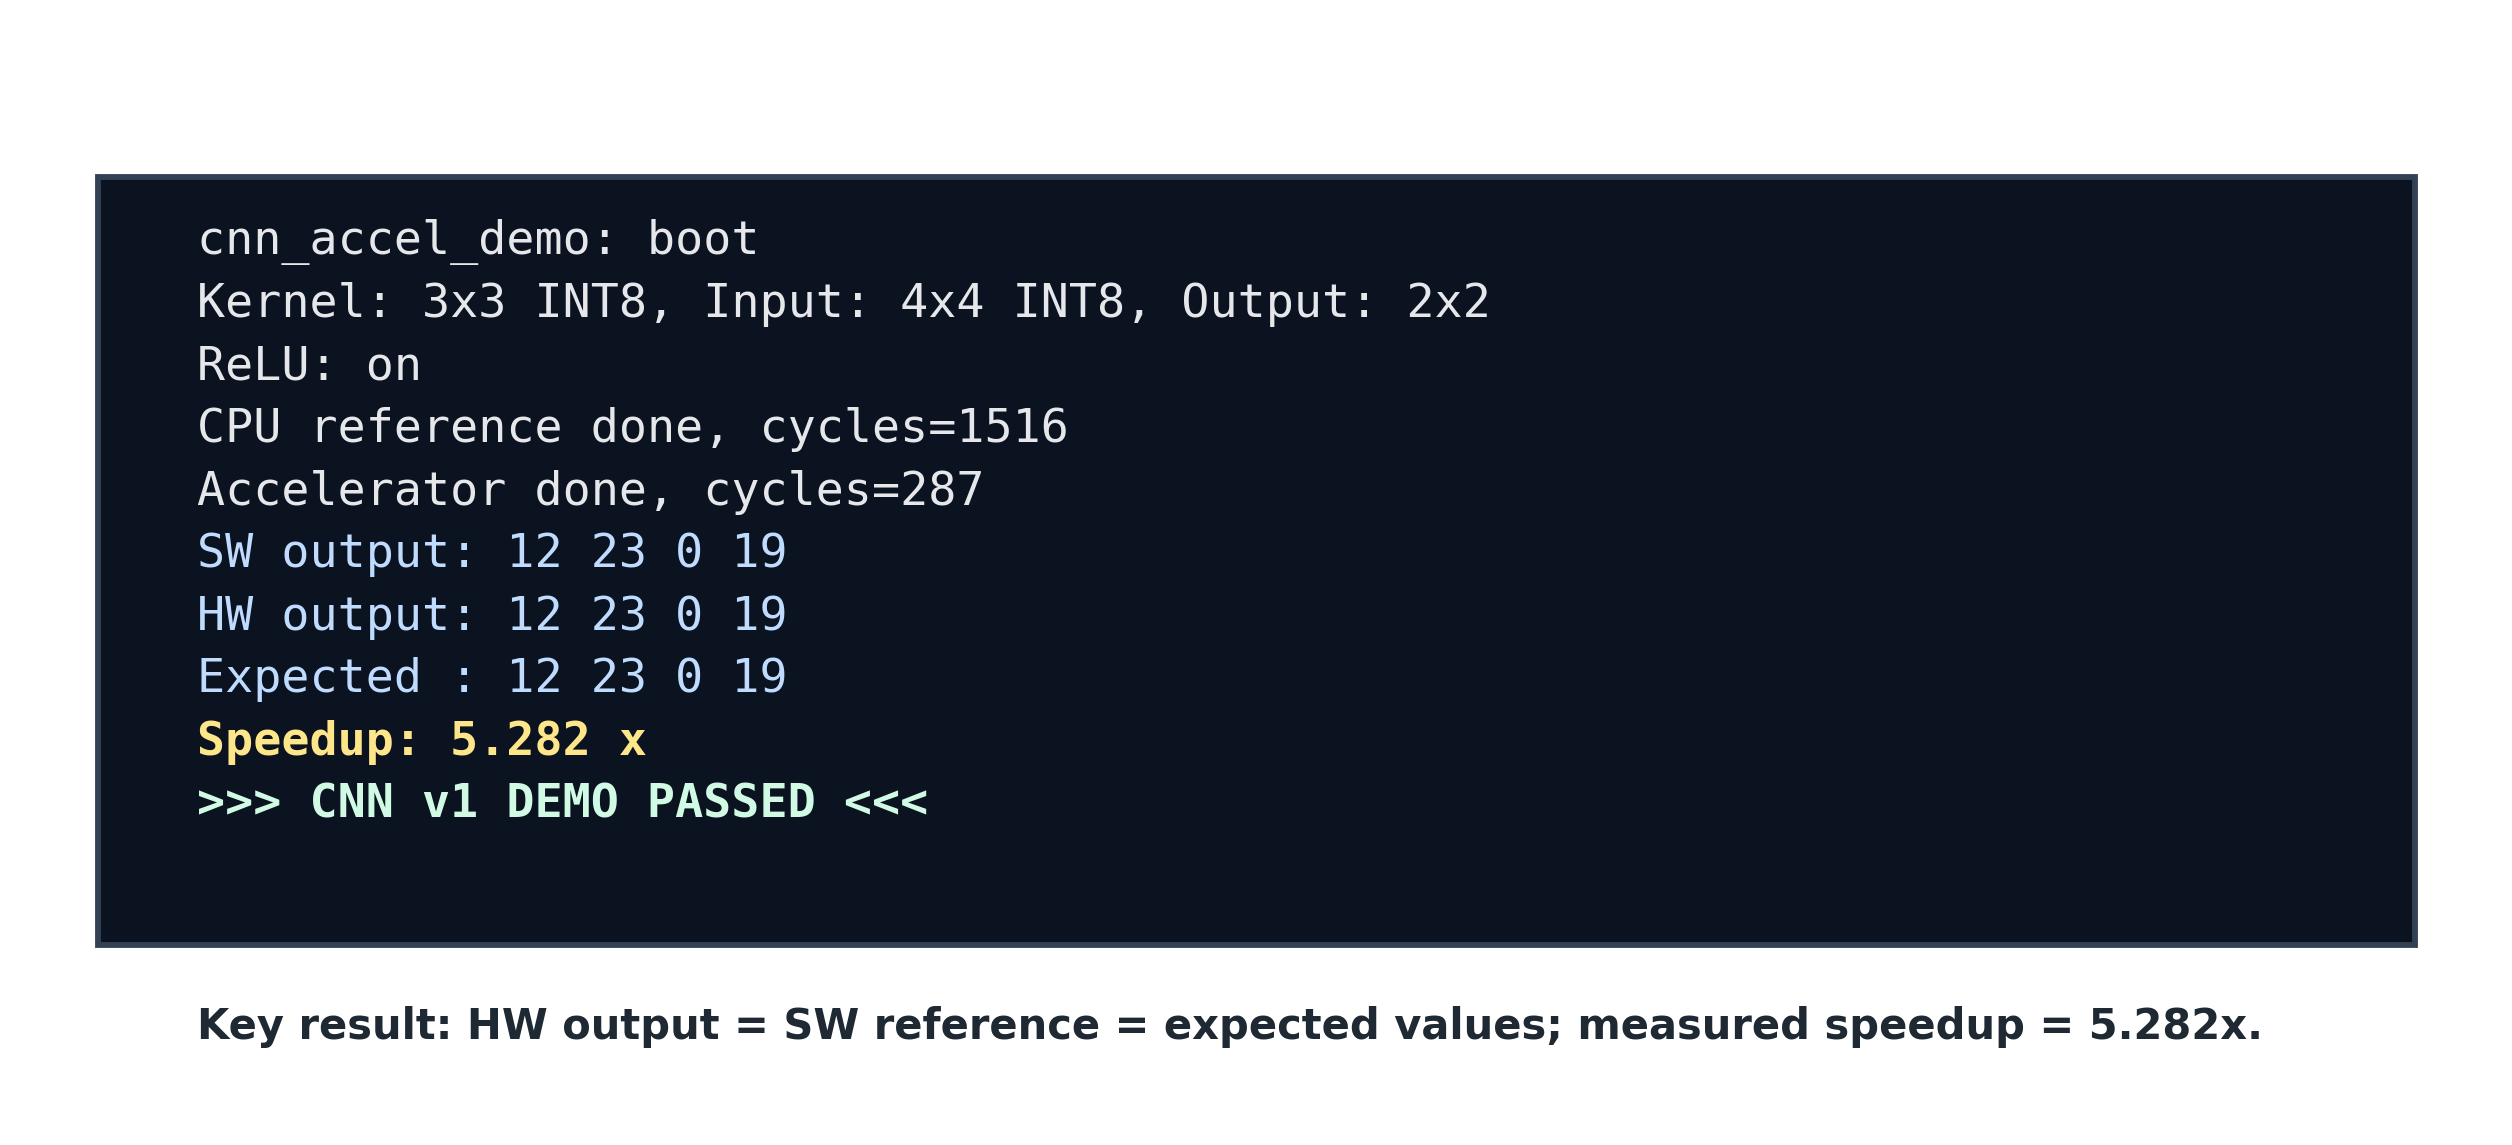
\includegraphics[width=0.85\textwidth]{figures/fig4_4_uart_cnn_v1.png}
\caption[UART terminal output from the CNN v1 board regression]{UART terminal output from the CNN v1 board regression running on the FPGA. The recorded serial log shows the CPU reference, NICE hardware output, and expected output all matching as 12, 23, 0, 19; the same log reports 287 accelerator cycles versus 1,516 CPU cycles, giving a measured 5.282$\times$ convolution speedup.}
\label{fig:uart_output}
\end{figure}

\subsubsection{FPGA Deployment: LeNet-5 Inference}

The complete LeNet-5 firmware (v8) was deployed on the FPGA board using the \linebreak\texttt{cnn\_sysclk\_ila} build mode. Two issues were identified and resolved during iterative board testing:

\begin{itemize}
\item \textbf{Conv2 ReLU position (v6$\to$v8):} In version~v6, ReLU was applied per-channel inside the NICE-accelerated convolution function, i.e., after each of the 6 input channels for Conv2. The correct behavior applies ReLU only after the accumulated sum across all 6 channels. This caused information loss during multi-channel accumulation and limited accuracy to 7/10 on the 10-image test set.
\item \textbf{UART baud-rate divisor (v6$\to$v8):} The UART divisor was initially set to 27 (16~MHz / 28 = 571,428~baud) instead of the correct value 138 (16~MHz / 139 $\approx$ 115,200~baud), causing intermittent serial corruption.
\end{itemize}

After these corrections, the v8 firmware produced the UART output shown in Figure~\ref{fig:4_7}. The LeNet-5 network classified all 10 MNIST test images correctly (10/10 = 100\%), with predictions matching the ground-truth labels for digits 7, 2, 1, 0, 4, 1, 4, 9, 5, and 9. This result confirms end-to-end correctness of the NICE-accelerated convolution pipeline on FPGA hardware.

\begin{figure}[htbp]
\centering
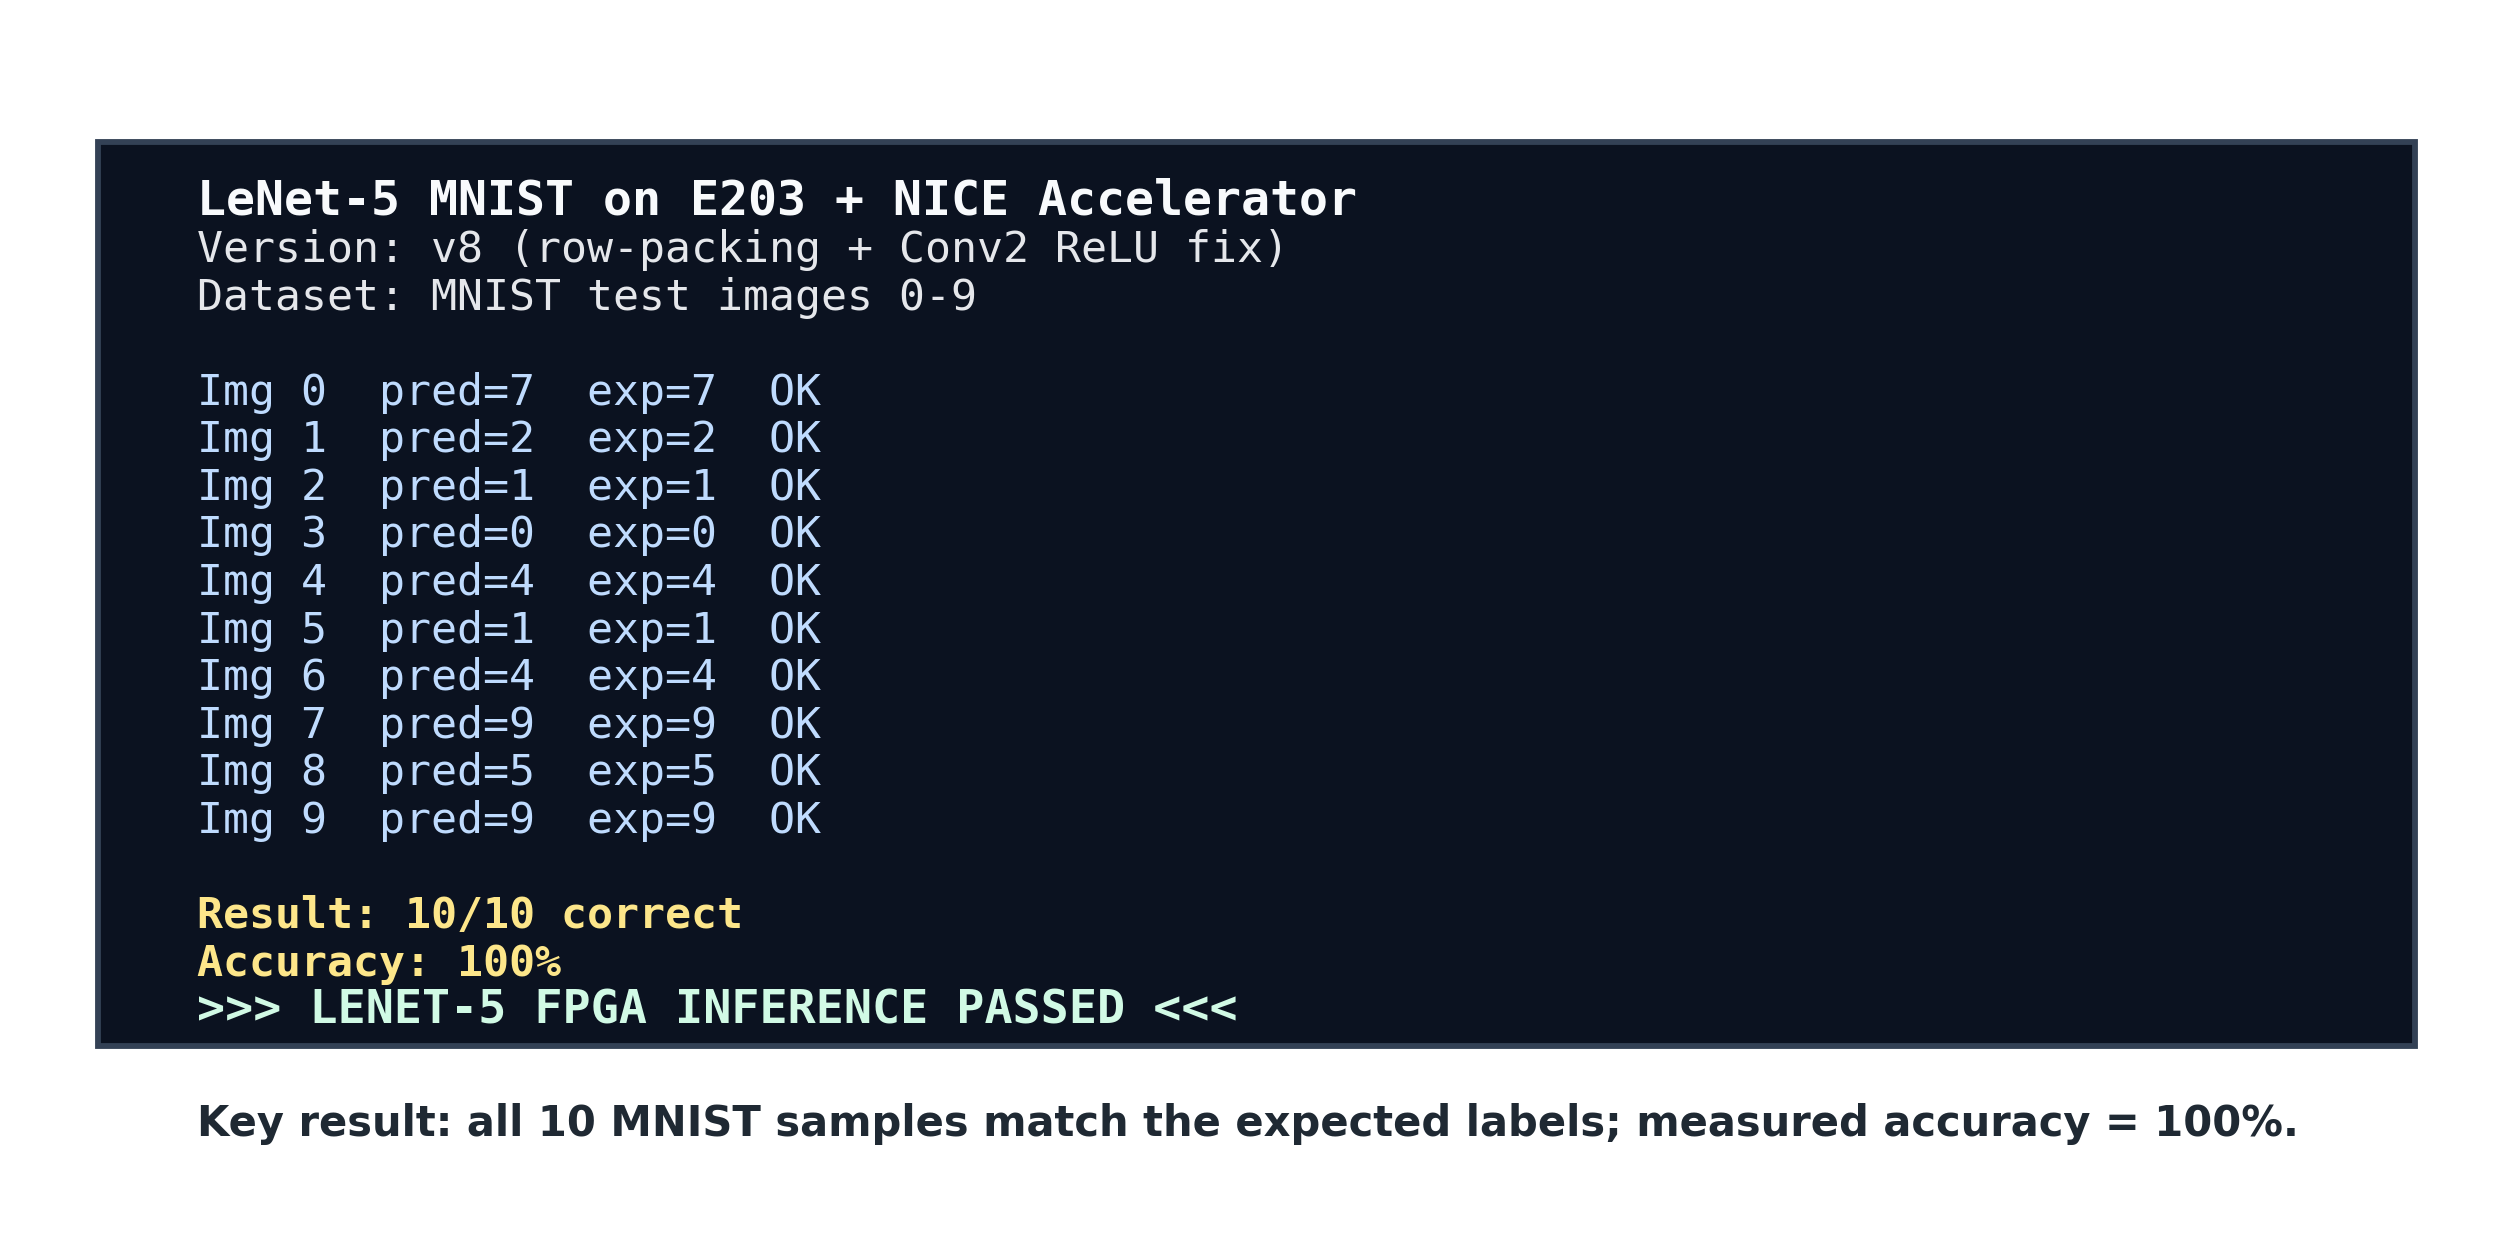
\includegraphics[width=0.85\textwidth]{figures/fig4_5_uart_lenet5.png}
\caption[UART terminal output from the LeNet-5 FPGA inference]{UART terminal output from the LeNet-5 MNIST inference running on the FPGA (v8, row-packing fix). All 10 test images are classified correctly (Img 0--9: 7, 2, 1, 0, 4, 1, 4, 9, 5, 9), demonstrating end-to-end correctness of the NICE-accelerated convolution pipeline.}
\label{fig:4_7}
\end{figure}

The board evidence therefore supports three claims: (1) the custom-instruction accelerator produces the correct convolution result matching the CPU reference; (2) the measured kernel execution is 5.282$\times$ faster than the software baseline; and (3) the end-to-end LeNet-5 inference pipeline operates correctly on FPGA hardware.

\subsection{Performance Measurement}

The NICE-accelerated convolution was benchmarked against a pure software reference implementation. For a 3$\times$3 convolution on a 4$\times$4 input feature map:

\begin{itemize}
\item CPU-only (software): 1,516 clock cycles
\item NICE-accelerated (hardware): 287 clock cycles
\item Speedup: 5.28$\times$
\end{itemize}

\begin{figure}[htbp]
\centering
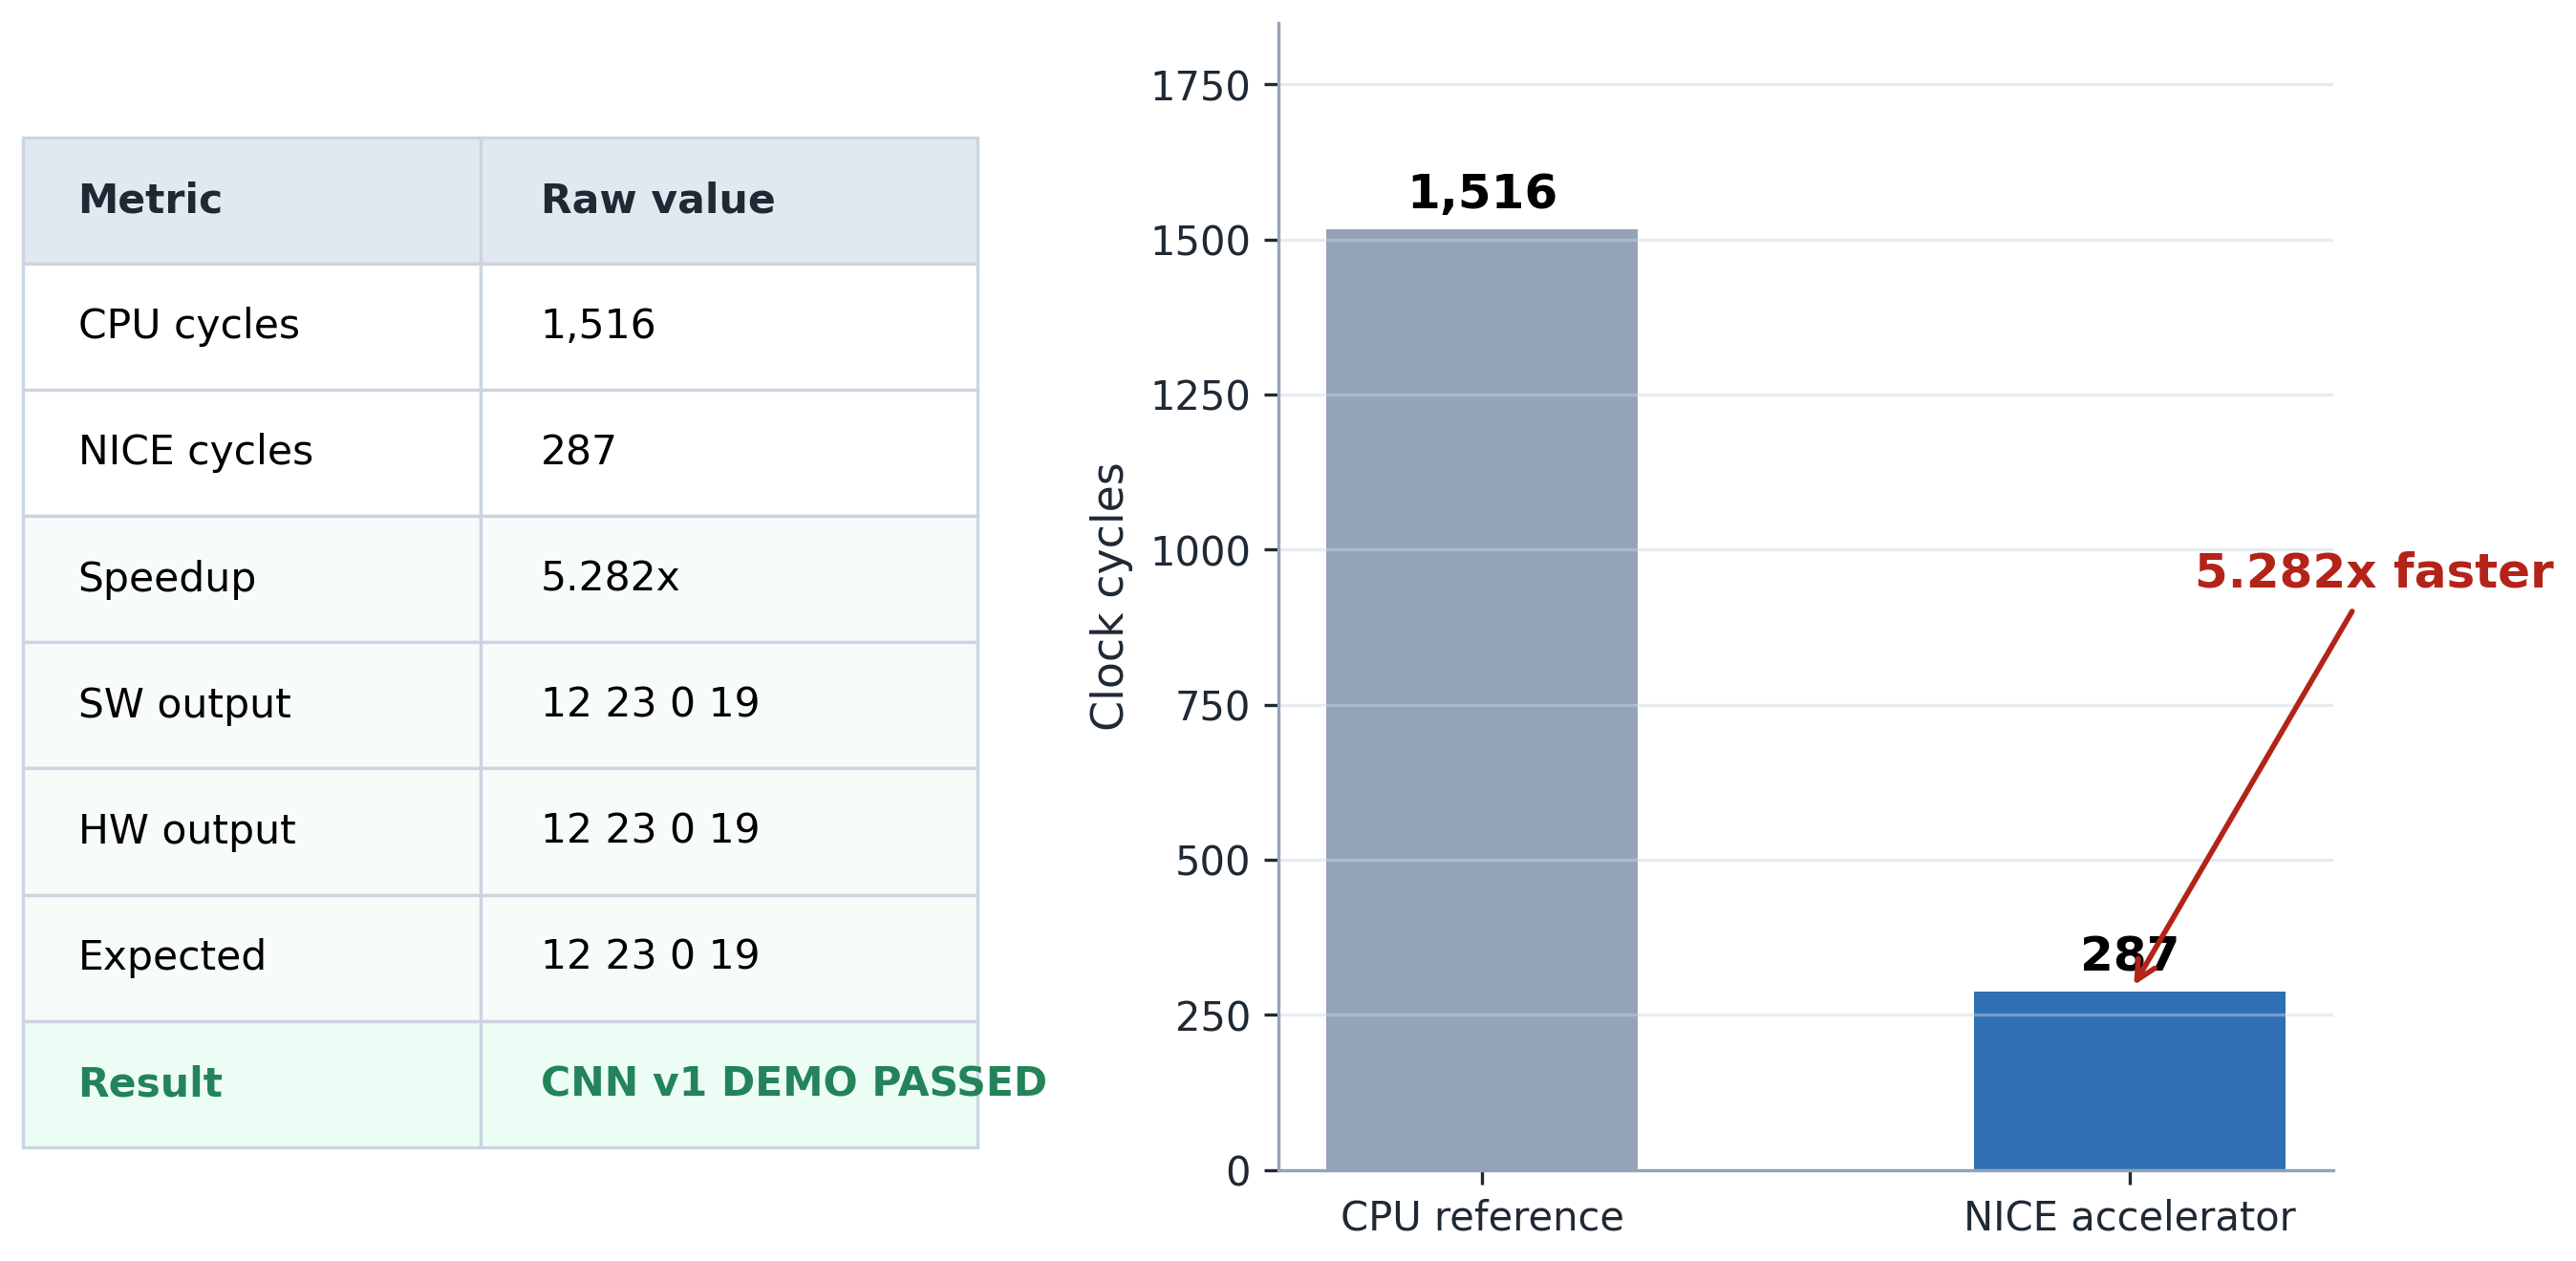
\includegraphics[width=0.75\textwidth]{figures/fig4_6_speedup_bar.png}
\caption{Measured convolution benchmark on the board demo: the NICE accelerator completes the test convolution in 287 cycles versus 1,516 cycles for the CPU reference, giving a 5.282$\times$ speedup.}
\label{fig:4_3}
\end{figure}

This measurement covers the convolution operation only: CLEAR, four WLOADs, four DLOADs, COMP, and RSTAT. The overall LeNet-5 inference time is dominated by the software FC layers, which perform approximately 50,000 multiply-accumulate operations per image at 16 MHz. The complete inference time per image is approximately 2--5 minutes in the current implementation, indicating that future work should target hardware acceleration of the FC layers, adoption of a Line Buffer architecture for pipelined data supply (as specified in the original task requirements), or migration to a reduced-precision FC datapath.

The measured 5.28$\times$ speedup (Figure~\ref{fig:4_3}) meets the design target of $\geq$5$\times$ acceleration for convolution operations.

\section{Resource Utilization}\label{sec:4_6}

The FPGA resource utilization for the complete E203 SoC with the CNN NICE accelerator is summarized in Table~\ref{tab:4_6} and Figure~\ref{fig:4_4} (post-implementation, \mbox{xc7a100t}).


\begin{table}[htbp]
\centering
\caption[FPGA resource utilization for the complete SoC]{FPGA resource utilization for the complete SoC with CNN NICE accelerator (post-implementation)}
\label{tab:4_6}
\begin{tabular}{lcccc}
\hline
Resource & Used & Available & Utilization (\%) \\ \hline\hline
LUT & 13,188 & 63,400 & 20.8 \\ \hline
LUTRAM & 219 & 19,000 & 1.2 \\ \hline
FF & 12,752 & 126,800 & 10.1 \\ \hline
BRAM & 35.5 & 135 & 26.3 \\ \hline
DSP & 0 & 240 & 0.0\tabularnewline
\multicolumn{4}{l}{\footnotesize DSP mapped to LUTs: 8-bit multipliers more efficient in fabric.} \\ \hline
BUFG & 5 & 32 & 15.6 \\ \hline
\end{tabular}
\end{table}

These figures demonstrate that the complete E203 SoC with CNN accelerator fits comfortably within the A7-100T device, leaving substantial headroom for future expansion.


\begin{figure}[htbp]
\centering
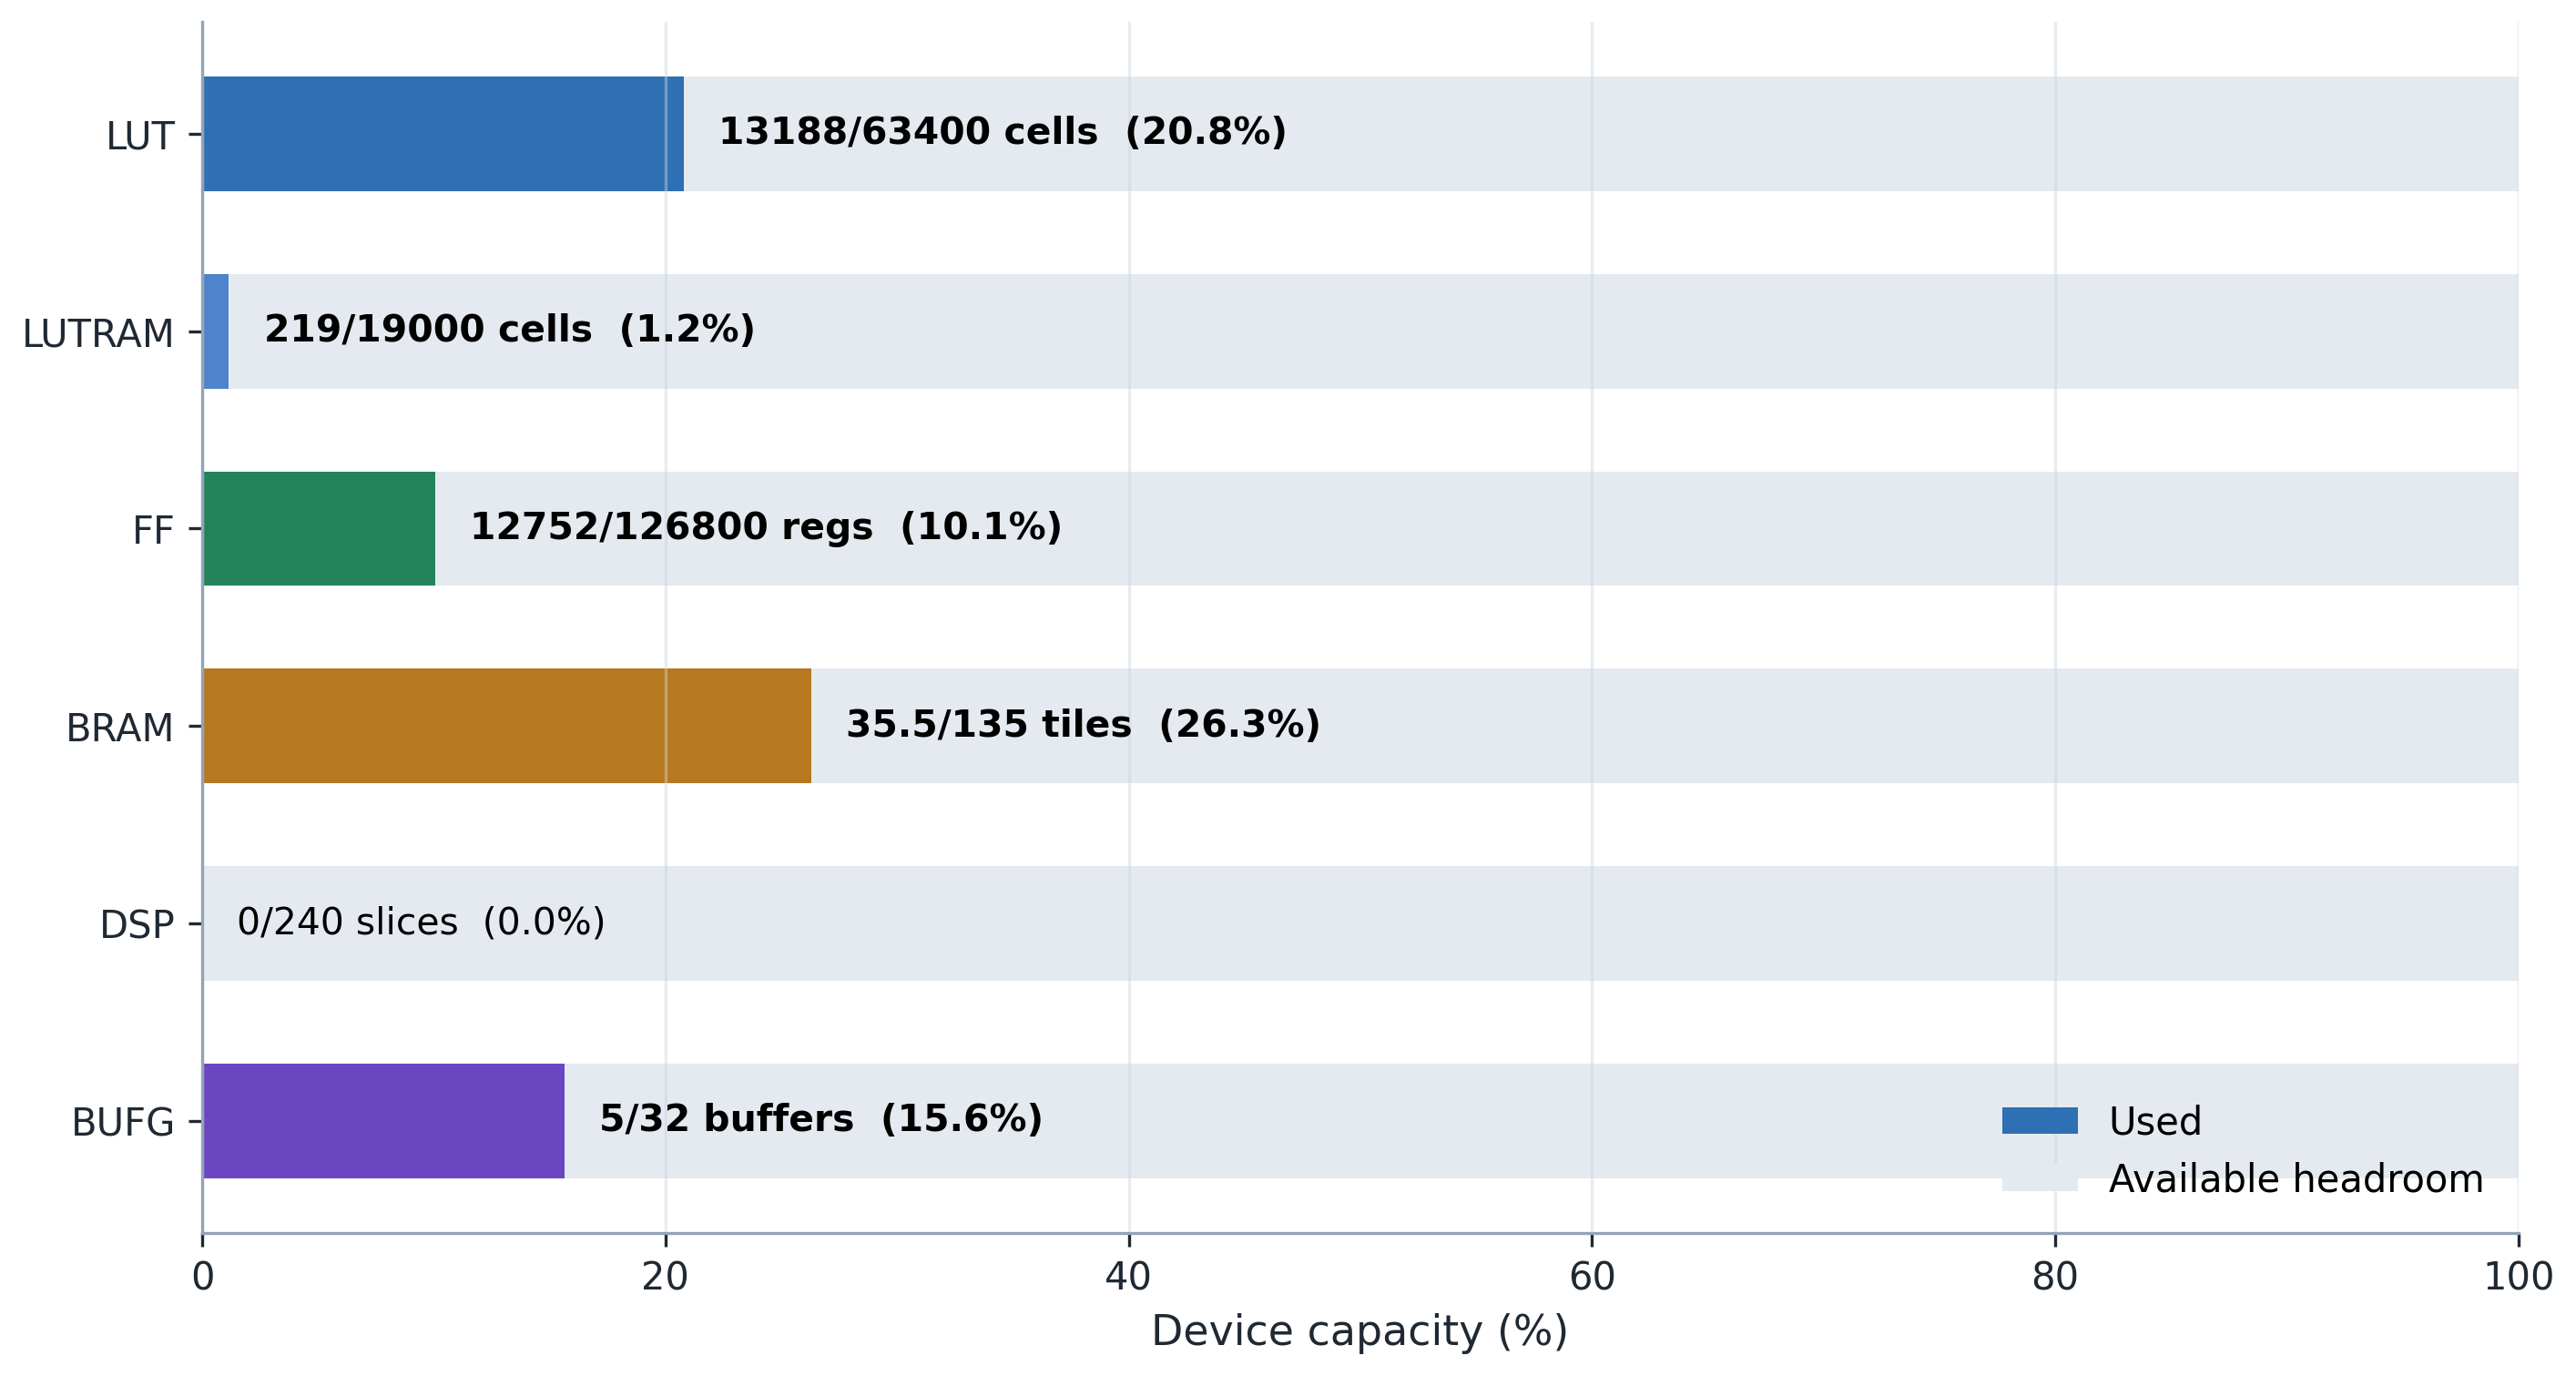
\includegraphics[width=0.70\textwidth]{figures/fig4_7_resource_pie.png}
\caption{FPGA resource-capacity fit for the complete E203 SoC with CNN NICE accelerator. Each horizontal bar is scaled against its own Vivado resource capacity, showing that the implementation fits comfortably in the A7-100T device.}
\label{fig:4_4}
\end{figure}

\begin{figure}[htbp]
\centering
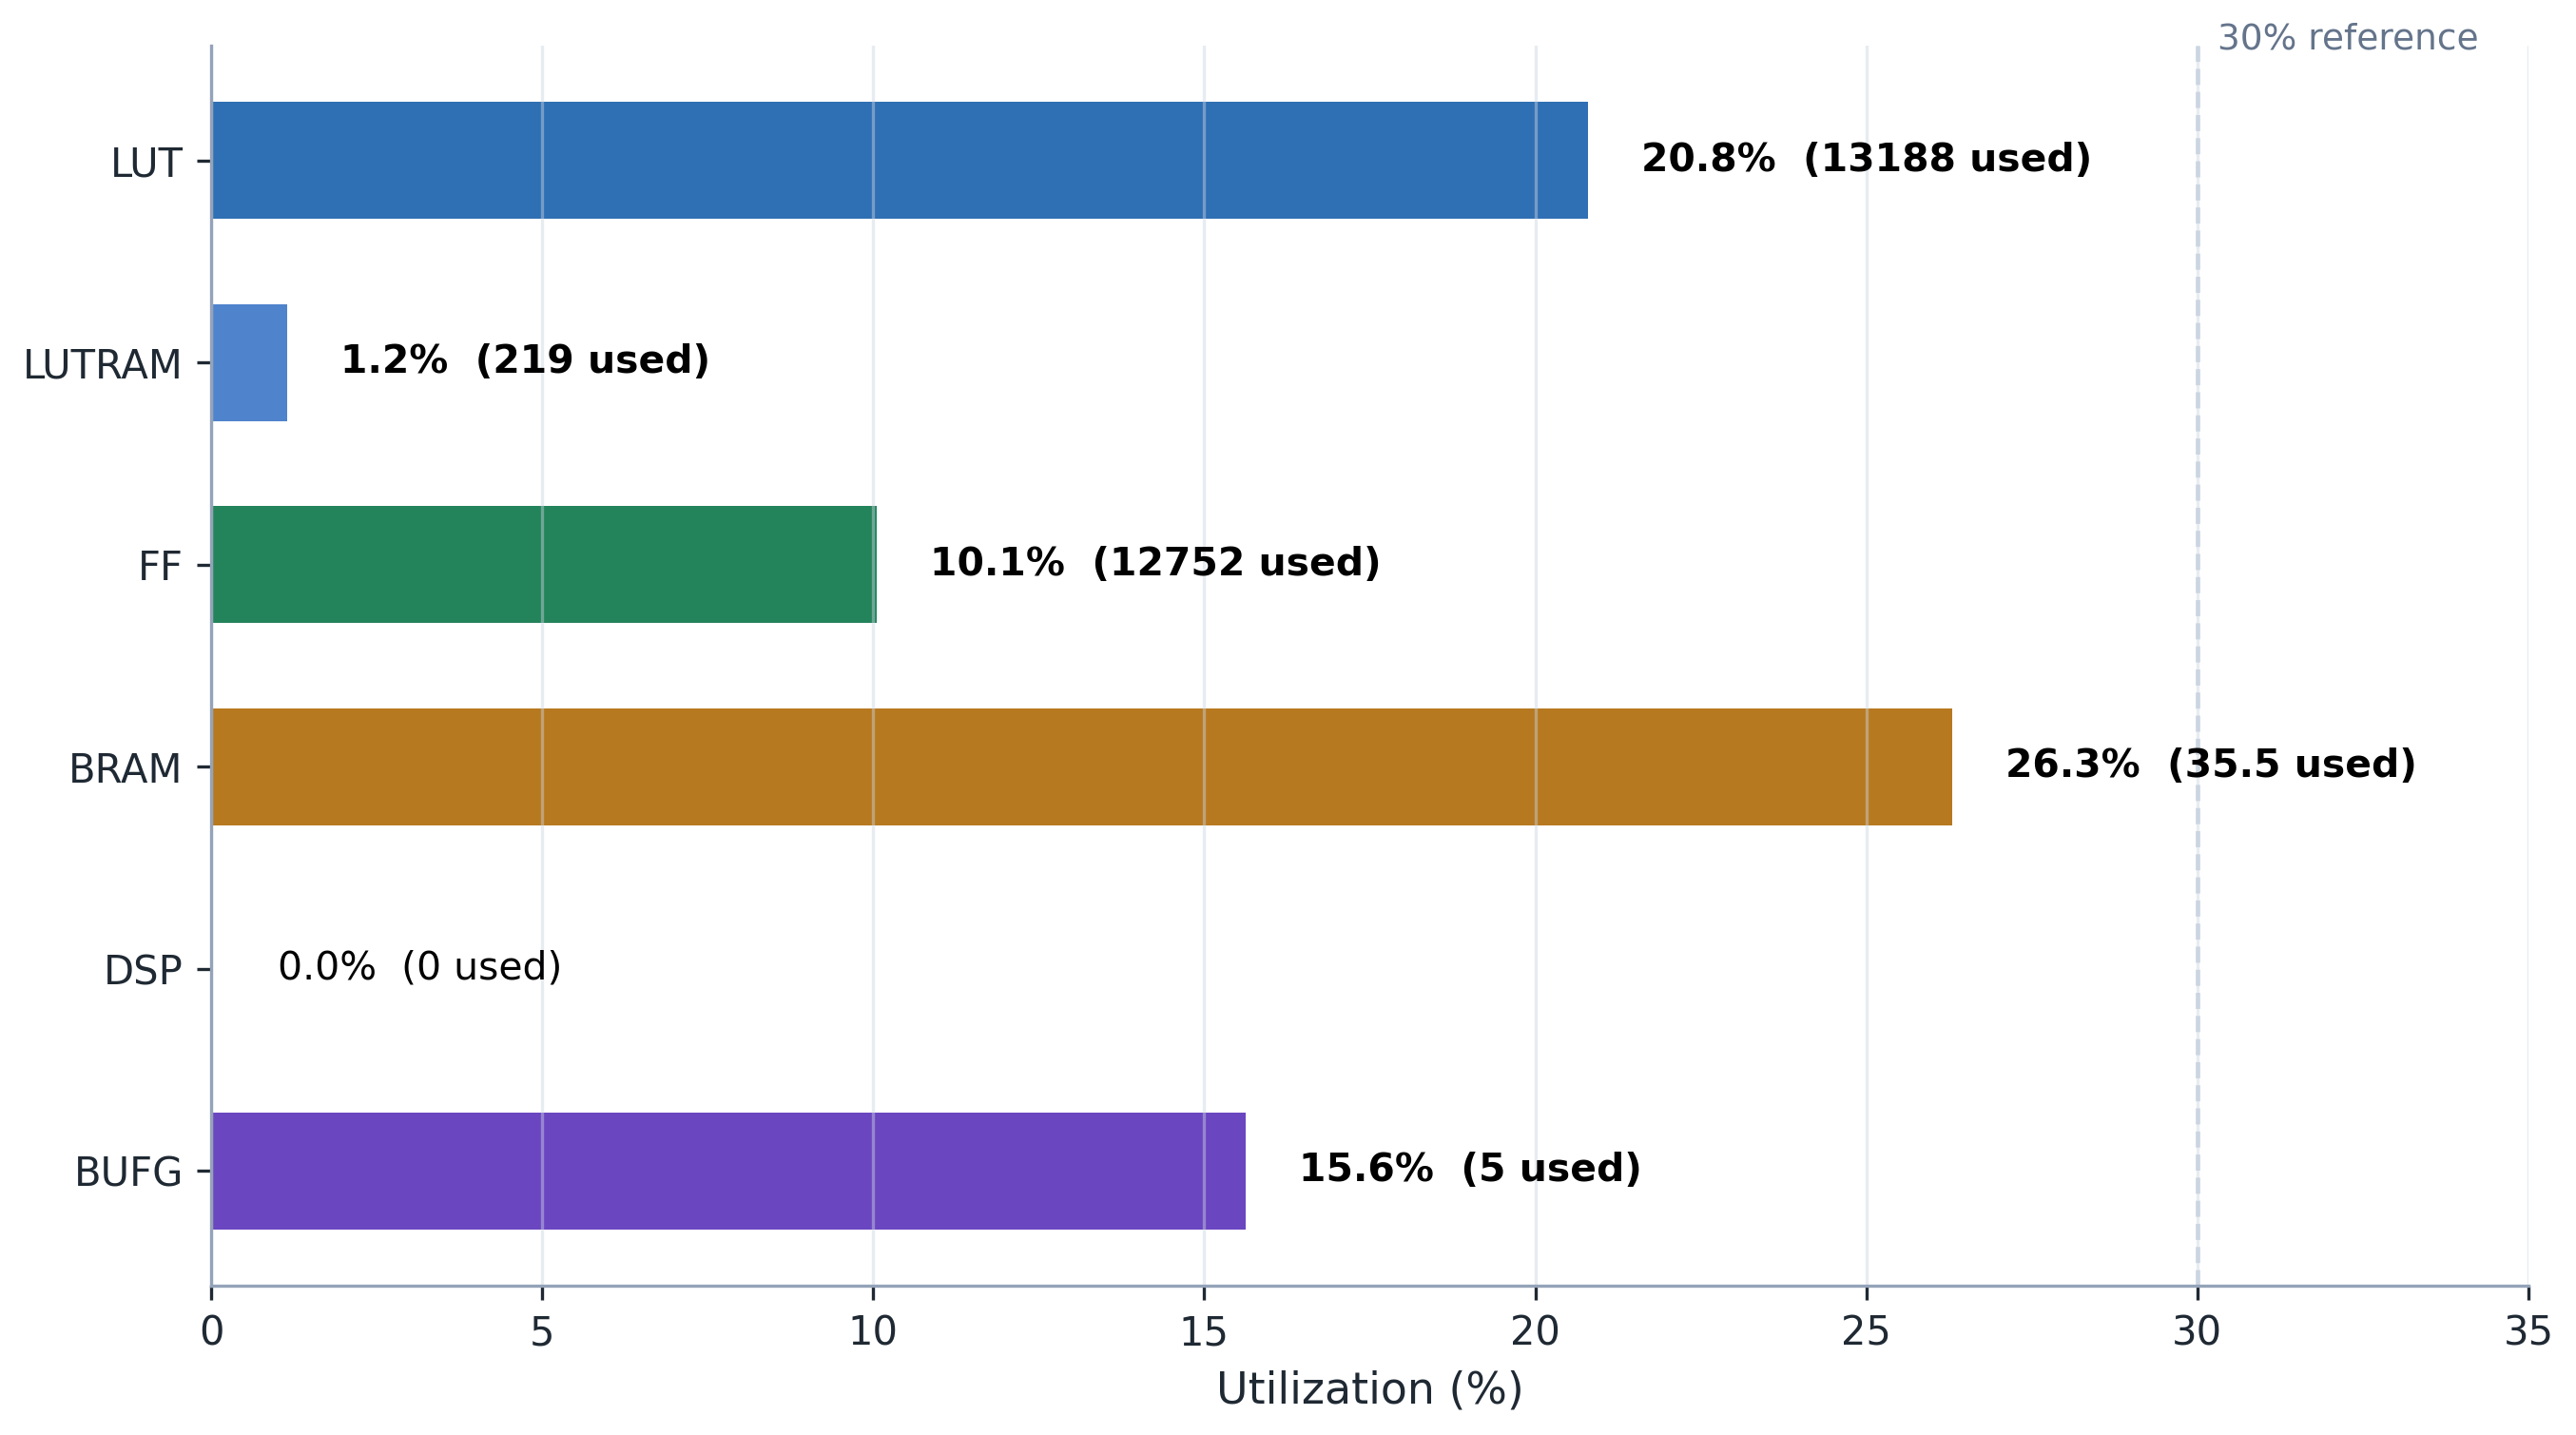
\includegraphics[width=0.75\textwidth]{figures/fig4_8_utilization_bar.png}
\caption{FPGA utilization by resource type for the complete SoC. LUT, FF, BRAM, DSP, and clock-buffer usage leave headroom for future accelerator expansion.}
\label{fig:4_5}
\end{figure}

\begin{figure}[htbp]
\centering
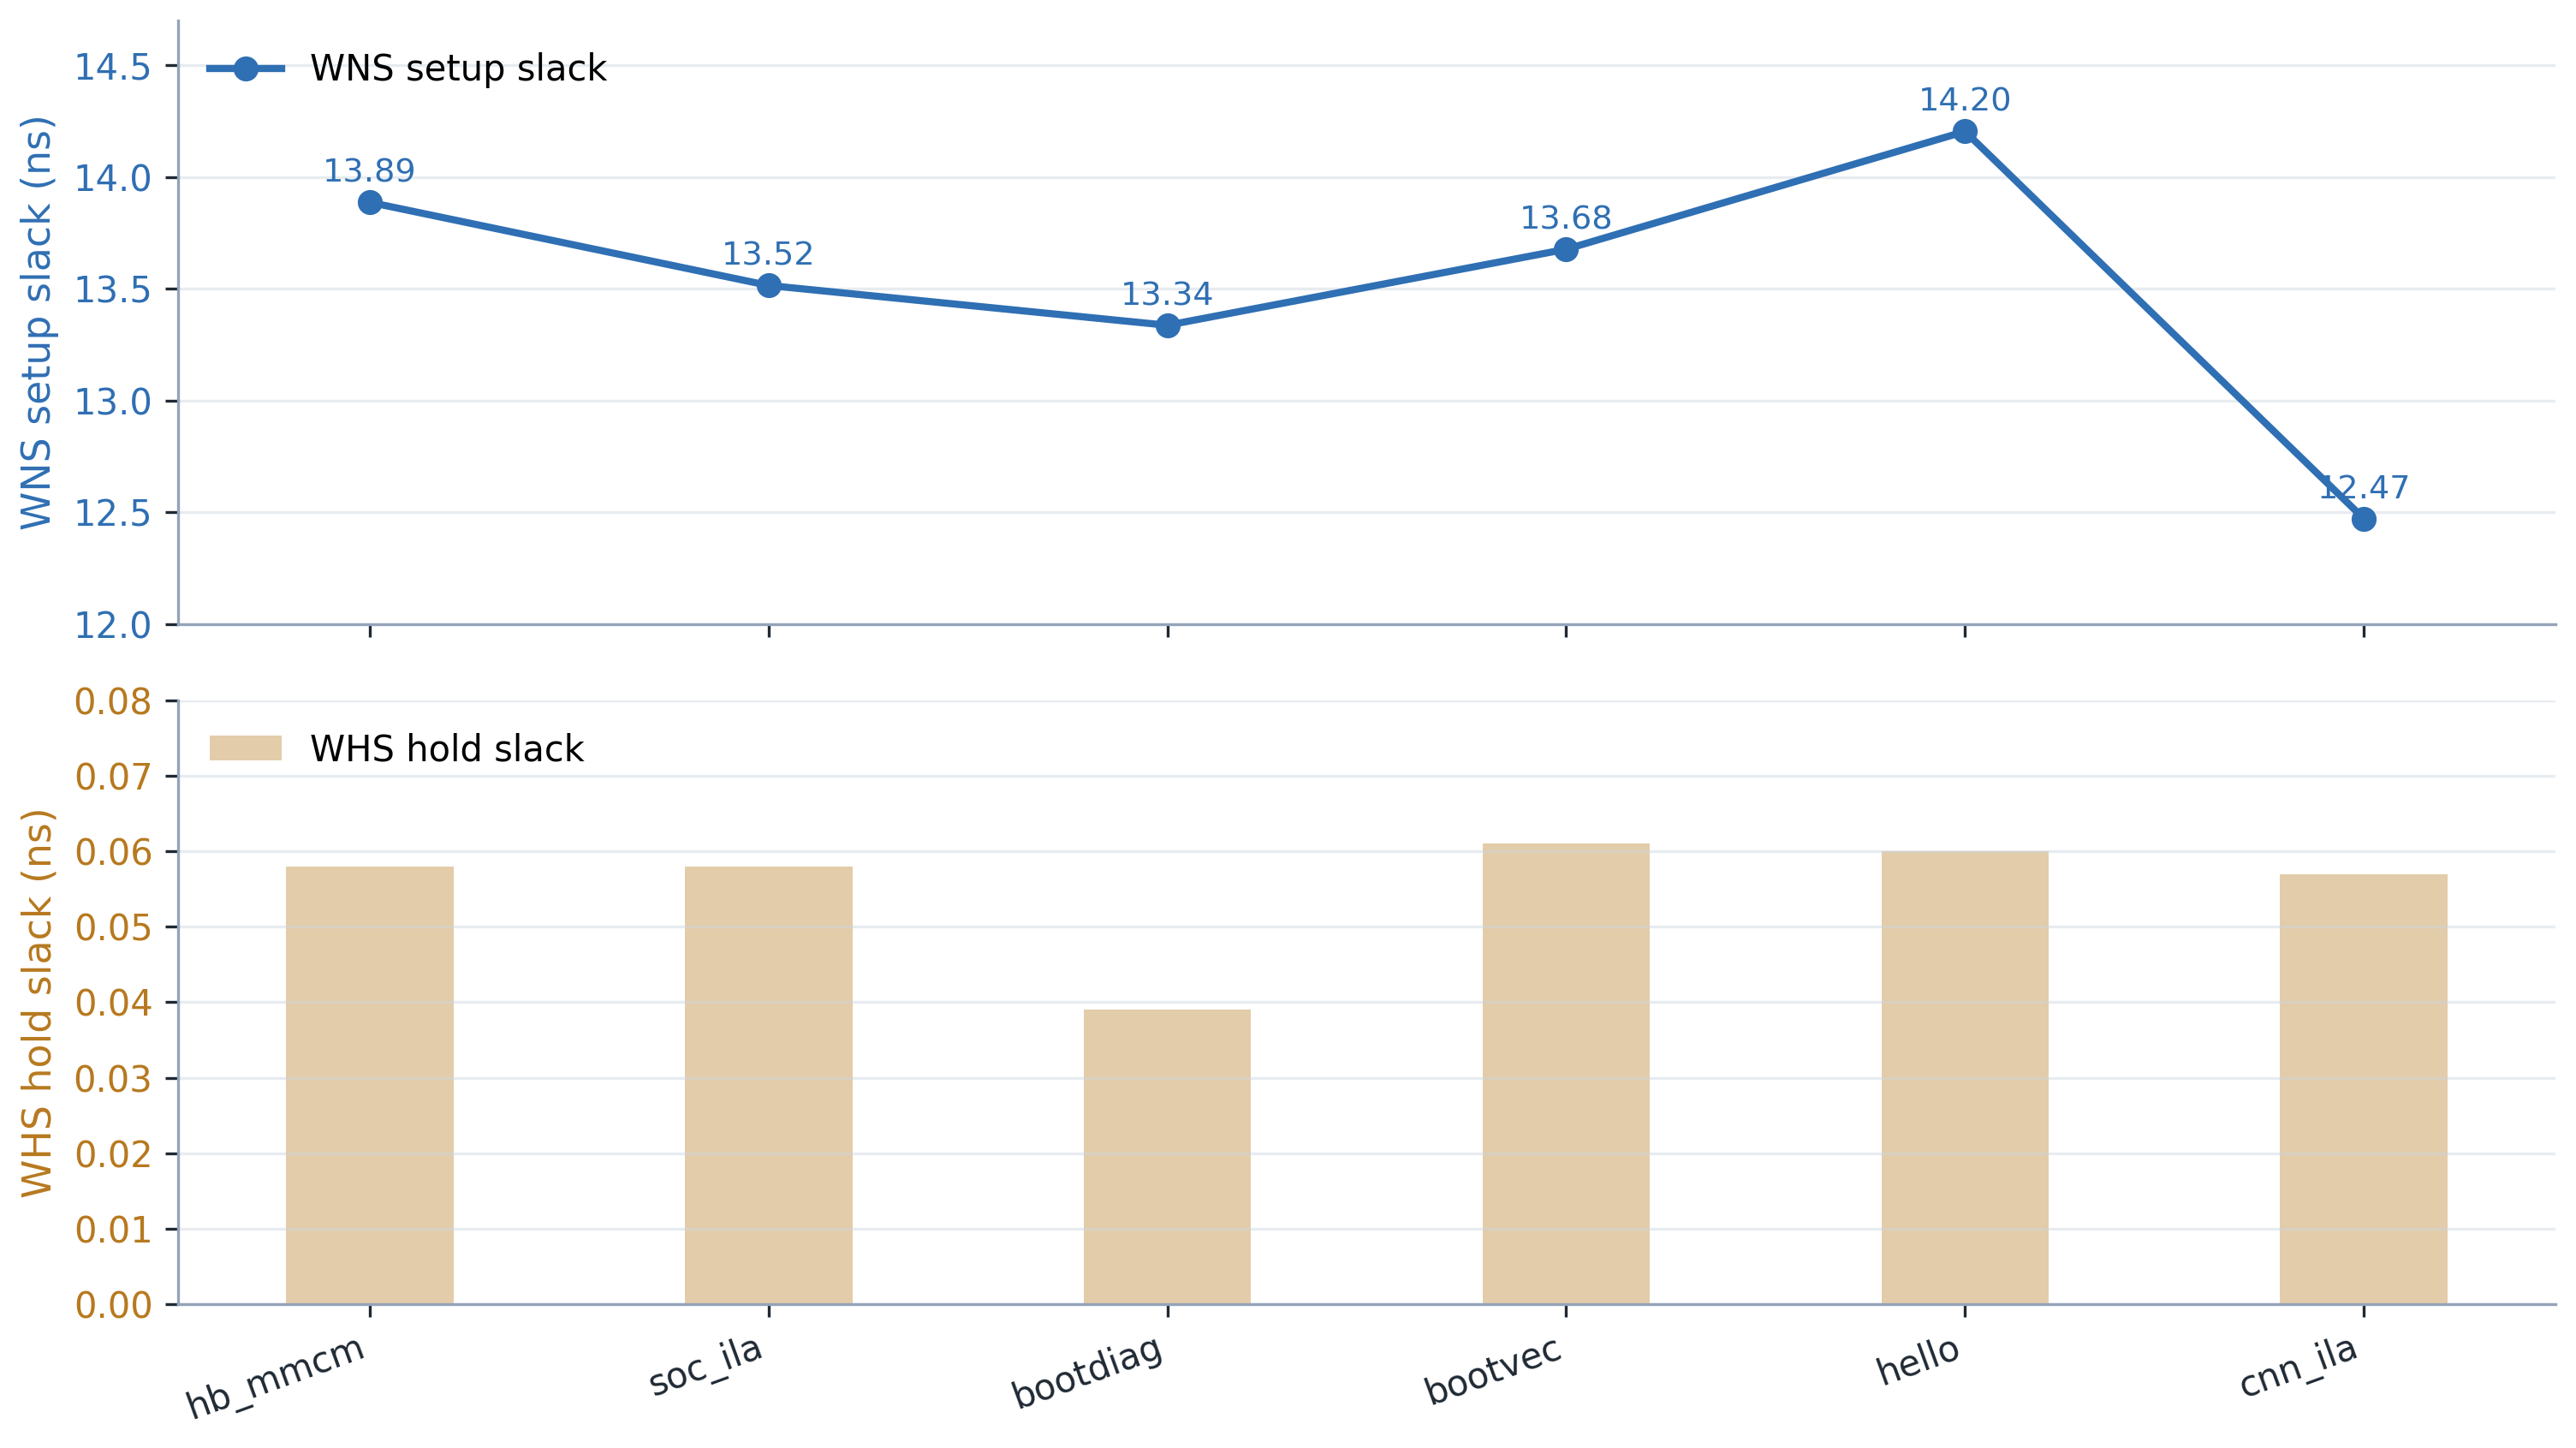
\includegraphics[width=0.80\textwidth]{figures/fig4_9_timing.png}
\caption{Timing closure summary across diagnostic and CNN board build configurations; all recorded builds meet setup and hold timing with positive slack.}
\label{fig:4_6}
\end{figure}
